\documentclass{article}

\title{CEE 498 SIS Project: Part IV \\ Electric Utility Design}
\date{2016/12/14}
\author{Steven Cai, Haitham El Mengad, Ketong Xie}

\usepackage{amsmath}
\usepackage{mathtools}
\usepackage[numbered,framed]{matlab-prettifier}
\usepackage{graphicx}
\usepackage{fancyhdr}
\usepackage{parskip}
\usepackage{geometry}
\usepackage{hyperref}
\usepackage{float}
\usepackage{chappg}
\graphicspath{{images/}}

\pagestyle{fancy}
\fancyhf{}
\lhead{Part IV}
\rhead{SC, HEM, KX}
\rfoot{\thepage}



\geometry{letterpaper, left=1in, right=1in, top=1in, bottom=1in}

% How to format Matlab code
% \begin{lstlisting}[style=Matlab-editor]
% \end{lstlisting}
			
% How to call an image	
% \includegraphics[width=\textwidth]{fig1}

\begin{document}

\maketitle
\setcounter{section}{4}
\pagenumbering[\thesection]{bychapter}
% \pagenumbering{arabic}
% \setcounter{section}{1}

%%%%%%%%%%%%%%%%%%%%%%%%%%%%%%%%%%%%
\paragraph{Problem Statement}
	In this problem, an electric utility seeks to achieve an optimal system design based on three main objectives: expected cost, global warming potential (GWP), and cost variance. The utility currently has five generation sources: conventional coal, advanced coal, conventional natural gas, nuclear, and hydroelectric. It has the option to build four additional types of generation plants with a chosen capacity: advanced coal with carbon capture and storage (CCS), advanced combined cycle natural gas, wind, and solar. Lastly, it has available three demand-side management (DSM) programs that may be implemented, which include two energy efficiency approaches and a load control approach; DSM programs decrease demand for electricity, but cost money to implement.
	
	Each generation source has its own expected cost, variance, and emissions footprint. The goal of the utility is to ensure that electricity can be provided to meet demand in each of their six load blocks, which are non-contiguous hours sorted by demand. This analysis proposes a suggested design for the utility based on these three objectives, and also considers other potential factors, such as an emissions cap, carbon tax, effect of climate change on hydroelectric generation, and technological advance in CCS.
	
	All tables are presented in the Tables section following this text. Figures are embedded inline below, but are presented in larger sizes in the Figures section following this text. The terms GWP, GHG (greenhouse gases), and emissions are used interchangeably in this text. Code in included in Appendix A.


%%%%%%%%%%%%%%%%%%%%%%%%%%%%%%%%%%%%
\paragraph{4.20}
	The utility has 61 decision variables, as follows:
	
	\begin{itemize}
		\item $x_{it}$: the power in megawatts (MW) for each plant per load block ($6 \times 9 = 54$ variables)
		\item $y_i$: design capacity of new plant $i$ in MW (4 variables)
		\item $z_k$: DSM implementation rate (3 variables)
	\end{itemize}
	


%%%%%%%%%%%%%%%%%%%%%%%%%%%%%%%%%%%	
\paragraph{4.21}
	The utility can choose to minimize total GWP in tons of carbon dioxide equivalents (CO2e) by using the following objective function:
	
	\begin{align*}
		% alt formulation with zk, unused
		%		min \  0.001 \sum_{i=1}^{I} g_i \Big[ \sum_{t=1}^{T} n_t \big( x_{it} - \sum_{k=1}^{K} z_k s_{kt}^{max} \big) \Big]
		% formulation with just x_it
		min \ 0.001 \sum_{i=1}^{I} \sum_{t=1}^{T} g_i n_t x_{it}
 	\end{align*}
 	 	
 	
	where: 
	\begin{itemize}
	\item $t$: load block index
	\item $i$: plant type index
	\item $T$: total number of load blocks (6) 
	\item $I$: total number of plant types (9)
	\item $g_i$: GWP for each type of power plant (kilograms [kg] CO2e per megawatt-hour [MWh])
	\item $n_t$: number of hours in each load block
	\end{itemize}
	
	Since $x_{it}$ has units of MW, the expression gives results in units of kg CO2e, which is multiplied by 0.001 to convert to metric tons (MT) of CO2e. $g_i$ and $n_t$ are given constants.
 		
 		
 		
 %%%%%%%%%%%%%%%%%%%%%%%%%%%%%%%%%%%%		
\paragraph{4.22}
	The utility can also minimize the expected annual cost of operation, which includes expected capital costs, expected variable operating costs, and expected DSM costs with the following objective function:
	
	\begin{align*}
		min \sum_{t=1}^{T} \bigg\{ 
		\sum_{i=1}^{I} \big( n_t x_{it} \bar{c}_i^v + 1000y_i \bar{c}_i^c \big)
		+ \sum_{k=1}^{K}  n_t \bar{c}_k^d z_k s_{kt}^{max}
		\bigg\}
	\end{align*}
		
	where:
	\begin{itemize}
		\item $k$: DSM program index
		\item $K$: total number of DSM programs (3)
		\item $\bar{c}_i^v$: mean variable cost of production for plant $i$ (\$/MWh)
		\item $\bar{c}_i^c$: mean annualized capital (fixed) cost for plant $i$ (\$/kilowatt [kW])
		\item $\bar{c}_k^d$: mean implementation cost for DSM program $k$ (\$/MWh)
		\item $z_k$: implementation rate for DSM program $k$ (proportion of $s_{kt}^{max}$)
		\item $s_{kt}^{max}$: maximum achievable energy savings for DSM program $k$ in load block $t$ (MW)
	\end{itemize}
	
	The first term $n_t x_{it} \bar{c}_i^v$ is the capital cost, the second term $1000y_i \bar{c}_i^c$ is the variable cost, and the third term $n_t \bar{c}_k^d z_k s_{kt}^{max}$ is the DSM cost for given $i$, $t$, and $k$.
	
	The unit balance for this expression is as follows:
	\begin{align*}
		\big( hr \times MW \times \frac{\$}{MWh} \big) + 
		\big( \frac{1000 \  kW}{MW} \times MW \times \frac{\$}{kW} \big) +
		\big( hr \times \frac{\$}{MWh} \times MW \big)
	\end{align*}
	
	Units balance to dollars, confirming that this is an expression of cost.
 	

%%%%%%%%%%%%%%%%%%%%%%%%%%%%%%%%%%%%
\paragraph{4.23}
	Load constraints mean that the supply of power must meet the load demanded during each load block, which is the load minus the load relief from DSM implementation. Load blocks are the total hours in each year sorted into blocks by magnitude. The load constraints are formulated as follows:
	\begin{align*}
		l_t - \sum_{k=1}^{K} z_k s_{kt}^{max} \leq \sum_{i=1}^{I} x_{it}, \forall t \in T
	\end{align*}
	
	where:
	\begin{itemize}
		\item $l_t$: load in power block $t$ (MW)
	\end{itemize}
	
	There are 6 load constraints - one for each power block $t$. Units are in MW.
	
	
%%%%%%%%%%%%%%%%%%%%%%%%%%%%%%%%%%%%	
\paragraph{4.24}
	Instantaneous capacity constraints mean that for any given plant and time, power generated must be below the derated capacity for each plant, which accounts for unplanned outages. Unplanned outage rates are given constants for each plant type. These constraints are formulated as follows:
	
	\begin{align*}
		x_{it} \leq (1 - o_i^u) x_i^{max}, \forall i \in I, \forall t \in T
	\end{align*}
	
	where:
	\begin{itemize}
		\item $o_i^u$: unplanned outage rate, $o_i^u \in [0,1]$		
	\end{itemize}
	
	There are $6 \times 9 = 54$ constraints, since this must apply for each $x_{it}$, of which there are 6 load blocks and 9 plants. Units are in MW.


%%%%%%%%%%%%%%%%%%%%%%%%%%%%%%%%%%%%
\paragraph{4.25}
	Minimum generation constraints require plants to be generating electricity greater than the must-run capacity of each plant in each load block. The constraints are formulated as follows:
	
	\begin{align*}
		x_i^{min} \leq x_{it}, \forall i \in I, \forall t \in T
	\end{align*}
	
	where:
	\begin{itemize}
		\item $x_i^{min}$: must run capacity of plant $i$ (MW)
	\end{itemize}
	
	There are $6 \times 9 = 54$ constraints, since this must apply for each $x_{it}$, of which there are 6 load blocks and 9 plants. Units are in MW.
	
	
%%%%%%%%%%%%%%%%%%%%%%%%%%%%%%%%%%%%
\paragraph{4.26}
	The new generation bounds similar to the instantaneous capacity constraints, but for the new plants that may be built, since the design capacity of a new plant, $y_i$, is a decision variable. These constraints state that the design capacity must be less than the maximum allowed capacity for its plant type, $x_i^{max}$, and restate the instantaneous capacity bounds with $y_i$ in place of $x_i^{max}$, as follows:
	
	\begin{align*}
		x_it &\leq (1-o_i^u) y_i &i \in [5, 8], \forall t \in T \\
		y_i &\leq x_i^{max} &i \in [5, 8]
	\end{align*}
	
	24 and 4 constraints, respectively, are defined by these inequalities. Units are in MW.
	
	
%%%%%%%%%%%%%%%%%%%%%%%%%%%%%%%%%%%%	
\paragraph{4.27}
	The complete optimization problem for minimum expected production costs is defined as follows:
	
	\begin{align*}
		min \sum_{t=1}^{T} \bigg\{ 
		\sum_{i=1}^{I} \big( n_t x_{it} \bar{c}_i^v + 1000y_i \bar{c}_i^c \big)
		+ \sum_{k=1}^{K}  n_t \bar{c}_k^d z_k s_{kt}^{max} 
		\bigg\}
	\end{align*}
	
	subject to:
	\begin{itemize}
		\item Load constraints (6)
		\item[] $l_t - \sum_{k=1}^{K} z_k s_{kt}^{max} \leq \sum_{i=1}^{I} x_{it}, \forall t \in T$
		\item Instantaneous capacity constraints (54)
		\item[] $x_{it} \leq (1 - o_i^u) x_i^{max}, \forall i \in I, \forall t \in T$
		\item Annual energy constraints - existing plants (5)
		\item[] $\sum_{t=1}^T n_t x_{it} - (1-o_i^p) 8766 x_i^{max} \leq 0, i = 1, 2, 3, 4, 9$
		\item Annual energy constraints - new plants (4)
		\item[] $\sum_{t=1}^T n_t x_{it} - (1-o_i^p) 8766 y_i \leq 0, i = 5, 6, 7, 8$
		\item Minimum generation constraints (54)
		\item[] $x_i^{min} \leq x_{it}, \forall i \in I, \forall t \in T$
		\item Bounds on DSM programs (6)
		\item[] $0 \leq z_k, \forall k \in K$
		\item[] $z_k \leq 1, \forall k \in K$
		\item New generation bounds (32)
		\item[] $x_{it} \leq (1-o_i^u) y_i, i \in [5, 8], \forall t \in T$
		\item[] $y_i \leq x_i^{max}, i \in [5, 8]$
		\item[] $0 \leq y_i, i \in [5,8]$
	\end{itemize}
	
	where:
	\begin{itemize}
		\item $o_i^p$: planned annual outage rate, $o_i^p \in [0, 1]$
		\item All other variables defined above.
	\end{itemize}
	
	There are a total of 161 constraints.
	
	
%%%%%%%%%%%%%%%%%%%%%%%%%%%%%%%%%%%%	
\paragraph{4.28}
	This section describes the minimum expected cost optimization problem.
	
	\subparagraph{Setup}
		The linear optimization problem defined in Part 4.27 was run in MATLAB using the \texttt{linprog} solver and the simplex algorithm. This required formulating the problem as follows:
		
	\begin{align*}
		\underset{x}{\min} \ f^T x \ 
		s.t. \Bigg\{ \substack{
		A \cdot x  \leq b \\
		Aeq \cdot x \leq beq \\
		lb \leq x \leq ub}
	\end{align*}
	
	where:
	\begin{itemize}
		\item $x$ is the 61-element column vector of decision variables, consisting of 54 $x_{it}$ variables, 4 $y_i$ variables, and 3 $z_k$ variables.
		\item $A$ and $Aeq$ are the coefficient matrices containing expressions that form constraints corresponding to the element in column vectors $b$ and $beq$. The constraints from the previous section were rewritten as coefficients for each decision variable, and moved such that the coefficients were on the left and the constraint value on the right. In this case, there are no equality constraints so $Aeq$ and $beq$ are empty.
		\item $lb$ and $ub$ are the upper and lower bounds, respectively, on the corresponding decision variables.
	\end{itemize}
	
	Some constraints were formulated as inequalities in matrix $A$, while others have a more straightforward interpretation as bounds on decision variable values, which were formulated as upper and lower bounds. The result was a $39 \times 61$ matrix for $A$, which contained the following constraint groups that were formulated as inequalities:
	
	\begin{itemize}
		\item Load constraints (6)
		\item Annual energy constraints, existing (5)
		\item Annual energy constraints, new (4)
		\item New generation bounds (first 24 for the unplanned outage rate constraint)
	\end{itemize}
	
	The other constraints were formulated as upper and lower bounds:
	
	\begin{itemize}
		\item $x_{it}$ (54): Instantaneous capacity constraints (upper) and minimum generation constraints (lower)
		\item $y_i$ (4): New generation bounds (upper) and zero (lower)
		\item $z_k$ (3): value from zero to one
	\end{itemize}
	
	
	\subparagraph{Results}
	The \texttt{linprog} solver identified a solution for $x_{it}$, $y_i$, and $z_k$, as shown in Table 4.28a. As expected, the cheapest existing power sources, which included conventional coal, advanced coal, nuclear, and hydroelectric, were run the most in all load blocks. These effectively composed the baseload power sources. The conventional natural gas plant was run in the first two load blocks, which were those with the highest demand, a peaker plant to meet demand. 
	
	Since further power was needed in the first two load blocks, the new plant with the cheapest capital cost, the advanced combined-cycle natural gas plant, was built at a capacity of about 135 MW, which was sufficient to fulfill demand during the first two load blocks. The more expensive plants (advanced coal and the two natural gas plants) were not used in the latter load blocks. New advanced coal with CCS, wind, and solar plants were not constructed, partly due to their high capital costs, and demand was satisfied using other sources. 
	
	Lastly, load control was the only DSM program implemented (at 85\%), despite its higher cost, since it had the most reductions in the heaviest load block 1 (as shown by red arrow in Figure 2). Figure 1 shows the generation in all load blocks per plant type, and Figure 2 shows the generation contribution from each plant in each load block.
	
	\begin{figure}
		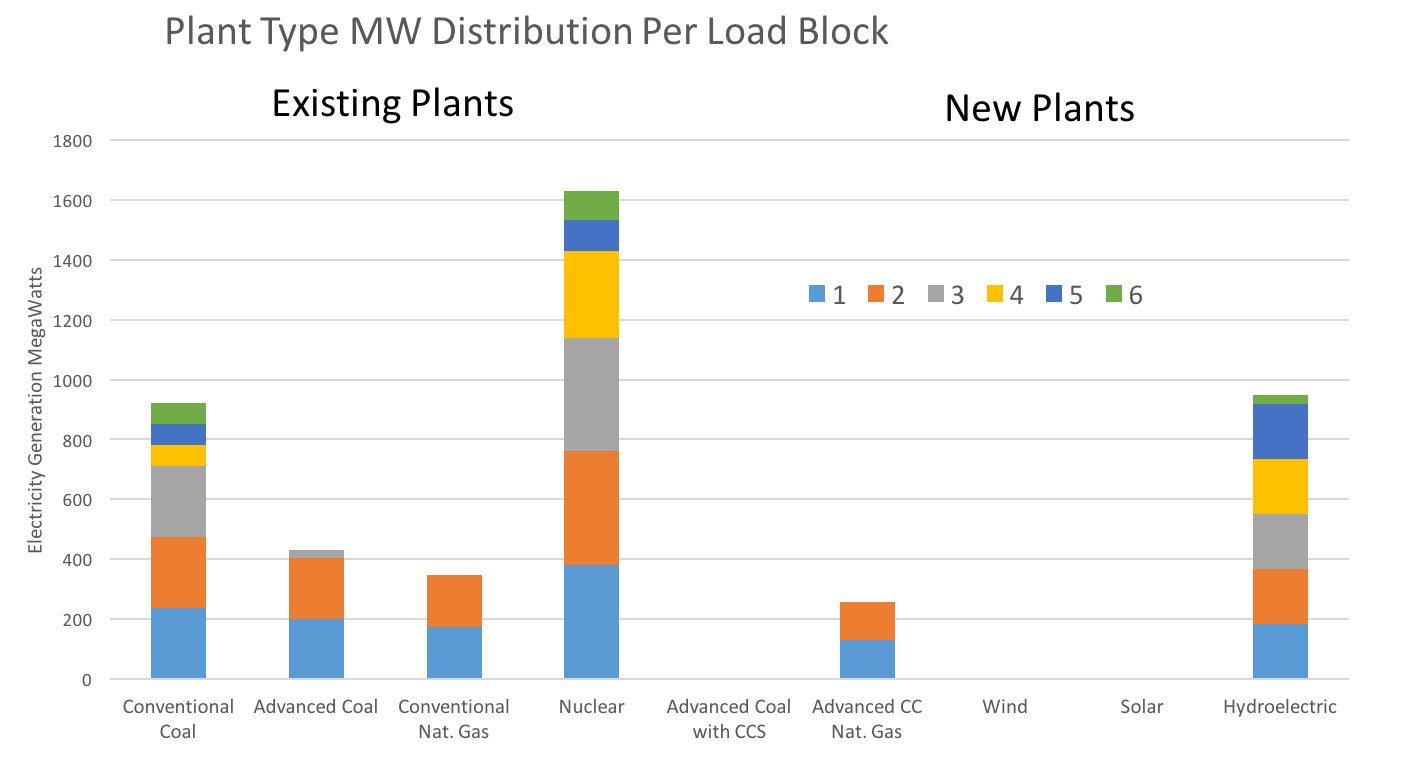
\includegraphics[width=\textwidth]{428_1_Mincostplantdis}
		\caption{Generation in each load block per plant.}
	\end{figure}
	
	\begin{figure}
		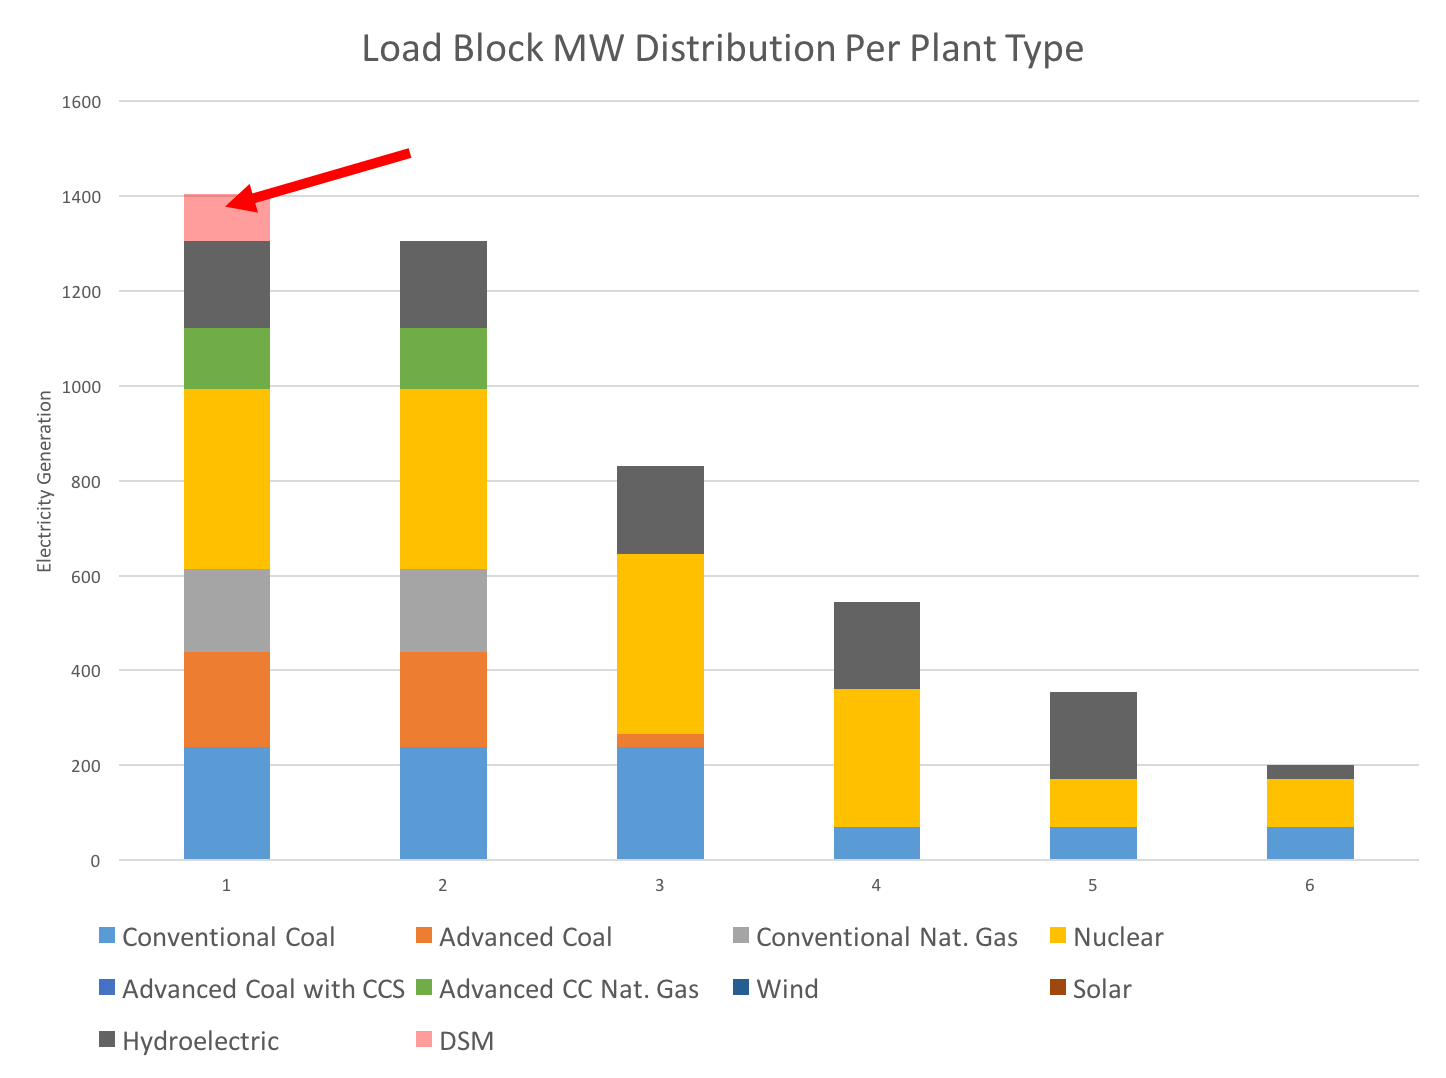
\includegraphics[scale=0.5]{428_2_Mincostloaddist}
		\centering
		\caption{Generation in each plant per load block. Red arrow shows the power demand removed by DSM.}
	\end{figure}
	
	The minimum expected cost is \$5.5031e+07, or about \textbf{\$55 million}. GWP from this solution is 1.0279e+06, or about \textbf{1.03 million MT} of CO2e. The cost variance is $\$^2 3.8897e+13$, which gives a cost standard deviation of \$6.2367e+06, or about \textbf{\$6.2 million}. The standard deviations of the variable operating cost, the new plant construction cost, and DSM program implementations cost were \$6.1816e+06, \$8.0968e+05, and \$1.7000e+05, respectively. Thus, variable cost has a considerably higher impact on the total cost variance than that of capital costs, which in turn has a more significant impact than DSM implementation cost. 

	\subparagraph{Binding Constraints and Sensitivity Analysis}
		Binding constraints were calculated by computing the slack, or the difference between $b$ and $A \cdot x$ or between the upper/lower bounds and $x$ for each decision variable. To deal with numerical instability, a small $\epsilon = 10^{-14}$ was introduced. Of the 161 total constraints, 76 were binding. The binding constraints and their interpretations are presented in Table 4.28b. 
		
		Generally speaking, constraints on baseload plants (nuclear, hydro, coal, etc.) held at the upper bound when they were being run at full bore during the heaviest load blocks. Constraints held at the lower bound in the lighter load blocks for peaker plants, such as natural gas and coal (to a lesser extent). Constraints held for certain decisions, such as not constructing advanced coal with CCS, wind, or solar, and not using DSM programs 1 and 2. The load constraint also held in blocks 3-5. 
		
		In order to asses the sensitivity of the design to various constraints, shadow prices were calculated for each constraint. One at a time, the value of each of the 161 bounds was perturbed by increasing by 0.01, and \texttt{linprog} was re-run. The shadow price was calculated by dividing the change in the total expected cost by the perturbation value of 0.01. The choice of value was made based on $z_k$, which ranges from 0 to 1 and therefore requires a relatively small perturbation. We found that for $x_{it}$ and $y_i$, the shadow price was generally proportional in the nearby orders of magnitude (i.e., we achieve the same shadow price when perturbing by 1 as with 0.01), so we let $z_k$ be the limiting factor selecting the perturbation value. The resultant shadow prices are shown in Table 4.28c.
		
		Magnitude of shadow prices were divided into four rough ranges, which are distinguished by color in the table, and are listed below with select constraints that fell within each range. Full presentation of all shadow prices is included in Table 4.28c.
		
		\begin{itemize}
		\item No change (no color): annual energy constraints, new generation bounds for lighter load blocks, select lower bounds, upper bounds for power generation of peaker plants in lighter load blocks.
		\item $ 0 - 10,000$ (yellow): load constraint in block 6, new generation bounds in lighter blocks, wind lower bounds.
		\item $ 10,000 - 100,000$ (green): load constraints, baseload lower bounds, wind and advanced coal with CCS lower bounds.
		\item $\geq 100,000$ (red): lower bounds for lighter blocks, DSM programs 1 and 2 lower bounds.
		\end{itemize}
		
		Generally, lower bounds have higher shadow prices than upper bounds. This makes sense because upper bounds are seldom reached, as shown in the binding constraints section. This solution chooses not to build several plants, not to use the first two DSM programs, and runs few plants in lighter load blocks. Thus, forcing any of these events to happen causes a disproportionately high effect on the cost. Figure 3 shows the ten most sensitive decision variables and their shadow prices.
		
	\begin{figure}
		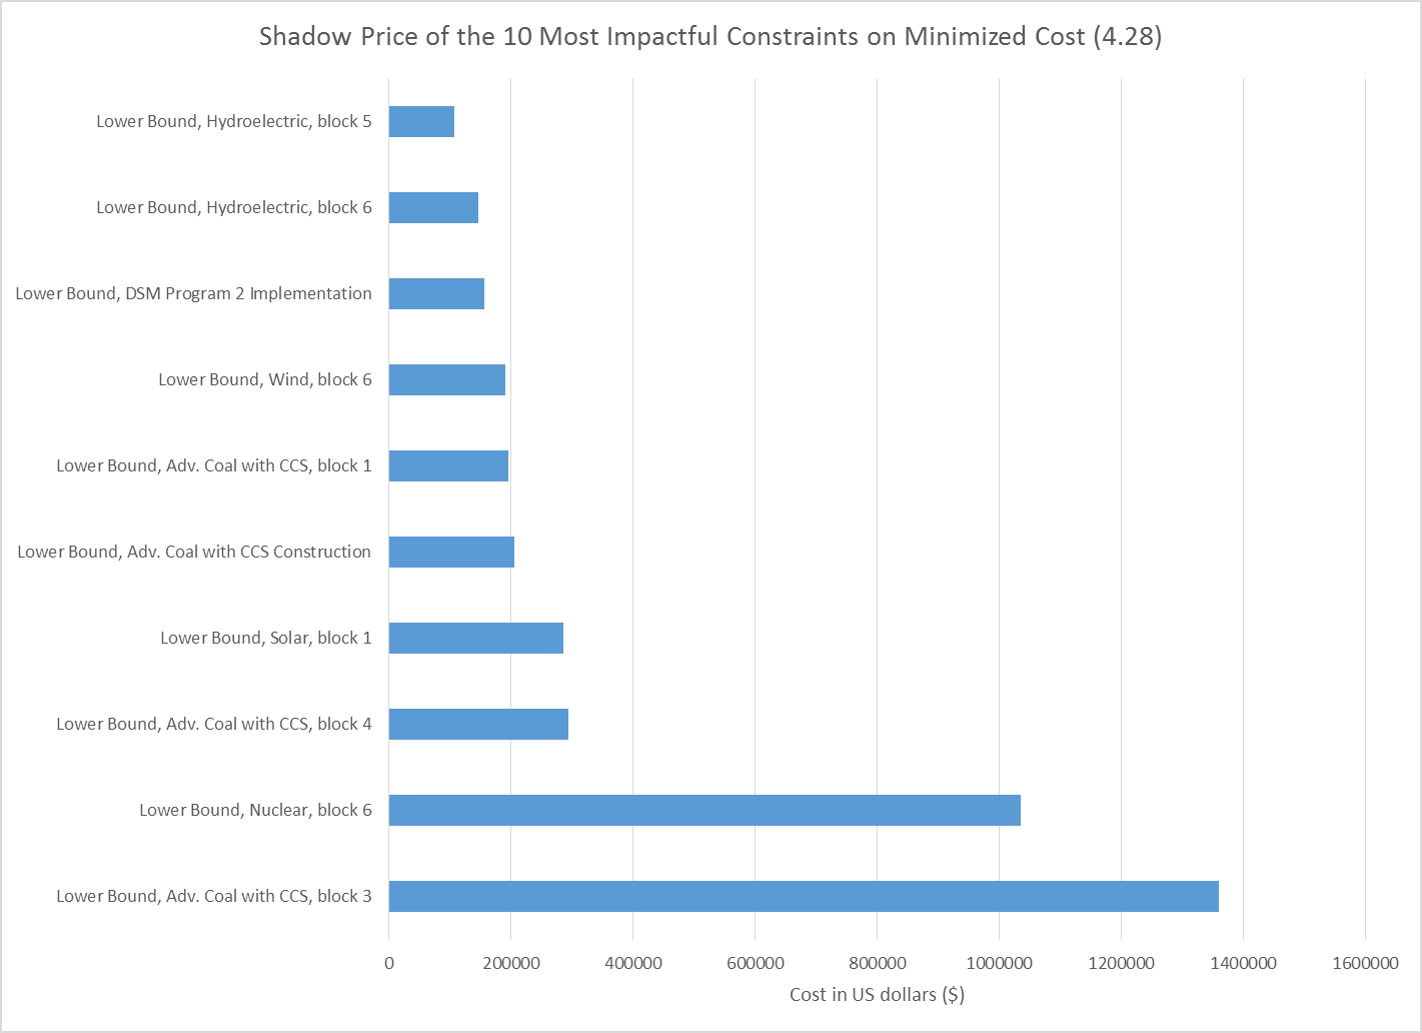
\includegraphics[width=\textwidth]{428_3_Mincostsens}
		\caption{Shadow price of most sensitive constraints.}
	\end{figure}


%%%%%%%%%%%%%%%%%%%%%%%%%%%%%%%%%%%%
\paragraph{4.29}
	This section describes the minimum GWP optimization problem.
	
	\subparagraph{Setup}
	The objective function described in Part 4.21 to find the minimum GWP was used with the same constraints developed for the minimum expected cost problem in Part 4.28 and solved using \texttt{linprog} as before. The only change is the objective function.
	
	\subparagraph{Results}
		As expected, power demands were met primarily through the three cleanest power plants: nuclear, solar, and wind, with contribution from hydroelectric in the first two load blocks to meet higher demand. Hydroelectric functions as a peaker plant in this solution, which is more consistent with smaller hydroelectric works (stream or penstock feed), or perhaps pumped storage solutions, than it is with large-scale hydroelectric works (dams). Since there is a minimum generation bound on conventional coal, this plant was run at the minimum capacity in each load block. No contribution from the other two advanced coal options or either natural gas option was used in generation. Since cost was not constrained, decision variables $y_i$ and $z_k$ were simply implemented at their maximum values - there is no cost penalty to doing so for the former, and the use of the latter reduces emissions through demand reduction. Figure 4 shows the generation contribution in all load blocks per plant type, and Figure 5 shows the generation contribution from each plant in each load block. Results are presented in Table 4.29a.
		
		\begin{figure}
			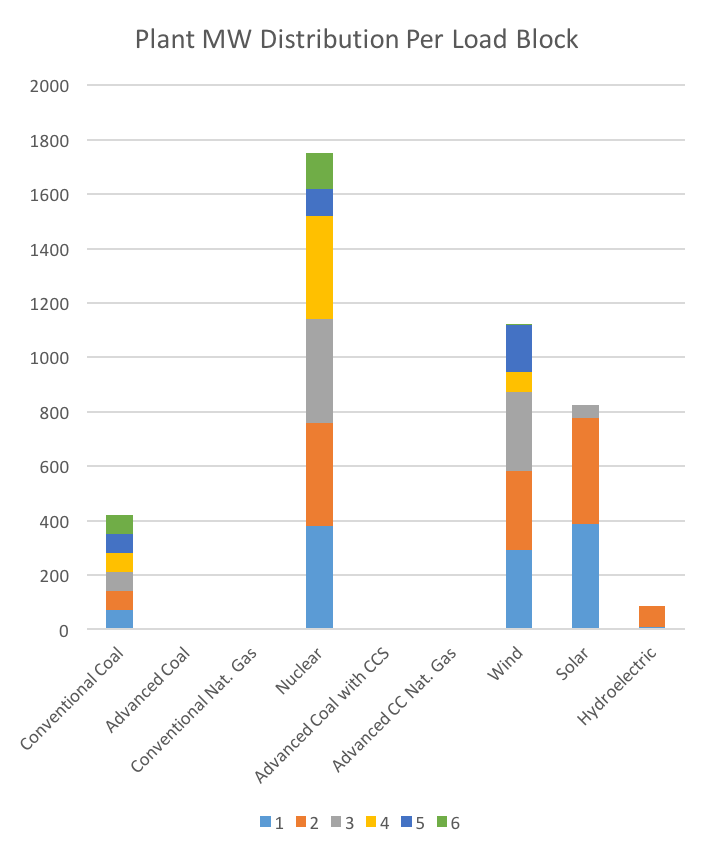
\includegraphics[scale=0.9]{429_4_Minemplantdist}
			\centering
			\caption{Generation in each load block per plant.}
		\end{figure}
		
		\begin{figure}
			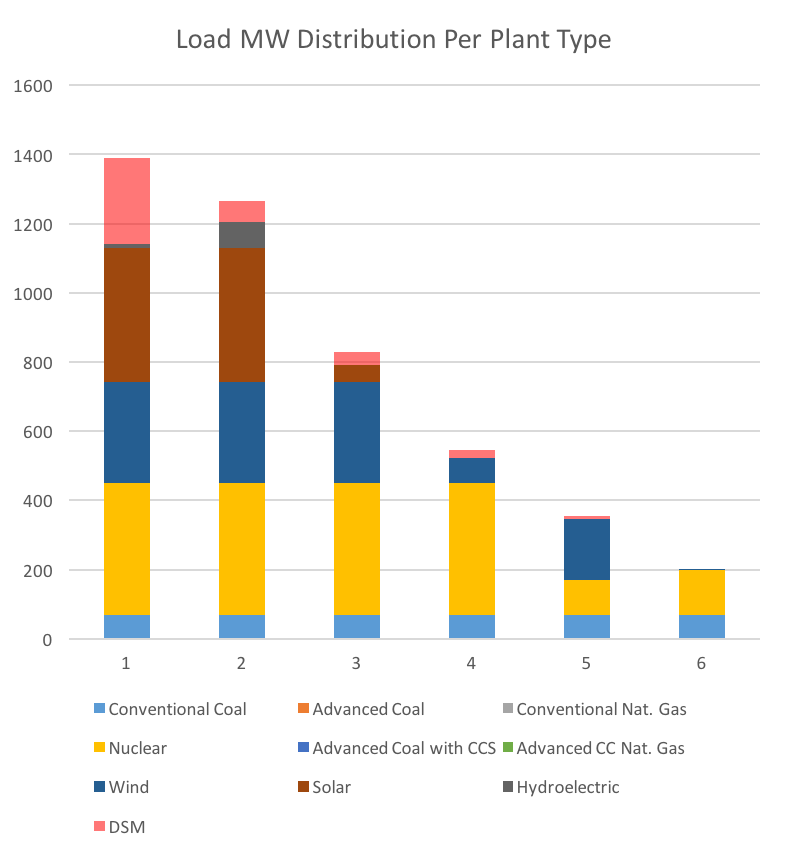
\includegraphics[scale=0.7]{429_5_Minemloaddist}
			\centering
			\caption{Generation in each plant per load block. Reductions in load from DSM programs are shown in red.}
		\end{figure}
		
		The expected cost for this solution is \$1.8392e+08, or about \textbf{\$184 million}, which is over three times the minimum cost. GHG emissions from this solution are 6.6282e+05, or about \textbf{663,000 MT} of CO2e, which is about 65\% of the emissions from the minimum cost solution. The cost variance is \$\$1.5361e+14, which gives a cost standard deviation of \$1.2394e+07, or about \textbf{\$12.4 million}, which is double that of the minimum cost solution. 
		
		The standard deviations of the variable operating cost, the new plant construction cost, and DSM program implementations cost were \$6.8061e+06, \$1.0306e+07 and \$2.5962e+05, respectively. This time, capital cost, instead of variable (operating) costs, is the driving factor in overall uncertainty. This makes sense because the uncertainties associated with construction of new plants should be much higher than that of operations (e.g., fuel price fluctuation). 
		
		In this solution, all plants were constructed. The higher standard deviation of this solution is reflected in the construction and use of wind and solar, which have a high standard deviations (capital and variable) and were not constructed in the minimum cost solution.
	
	\subparagraph{Binding Constraints and Sensitivity Analysis}
		Binding constraints were calculated with the slack method described in Part 4.28. Of the 161 total constraints, 62 were binding. Load constraints in the first 4 blocks were binding. Generally, minimum generation bounds held for all of the coal and natural gas plants, while maximum generation bounds were held for nuclear and wind, in particular. The maximum values for decision variables $y_i$ and $z_k$ were also selected. Binding constraints are presented in Table 4.29b.
		
		Shadow prices were calculated using the perturbation method described in Part 4.28. Magnitudes were again divided into four ranges, but they were of much smaller magnitude than in Part 4.28, indicating that the minimization of GWP is less sensitive than minimization of cost. Ranges and select decision variables in each range are:
		
		\begin{itemize}
			\item No change (no color): annual energy constraints, most upper bounds.
			\item $0 - 100$ (yellow): load constraints, lower bounds in load block 1.
			\item $100 - 1000$ (green): lower bounds in load blocks 2-4.
			\item $\geq 1000$ (red): lower bounds in lighter load blocks for coal and natural gas, DSM programs 1 and 2.
		\end{itemize}

		Again, DSM programs 1 and 2, and program 3 to a lesser extent, exhibited the greatest magnitude shadow prices. Additionally, lower bounds for emissions-heavy plants in the lighter load blocks impact the GWP significantly; turning on the most-polluting plants during the lighter load blocks, which also have the longest hours, significantly affects the solution. Figure 6 shows the 10 most significant shadow prices. Full results for shadow prices are presented in Table 4.29c.
		
		\begin{figure}
		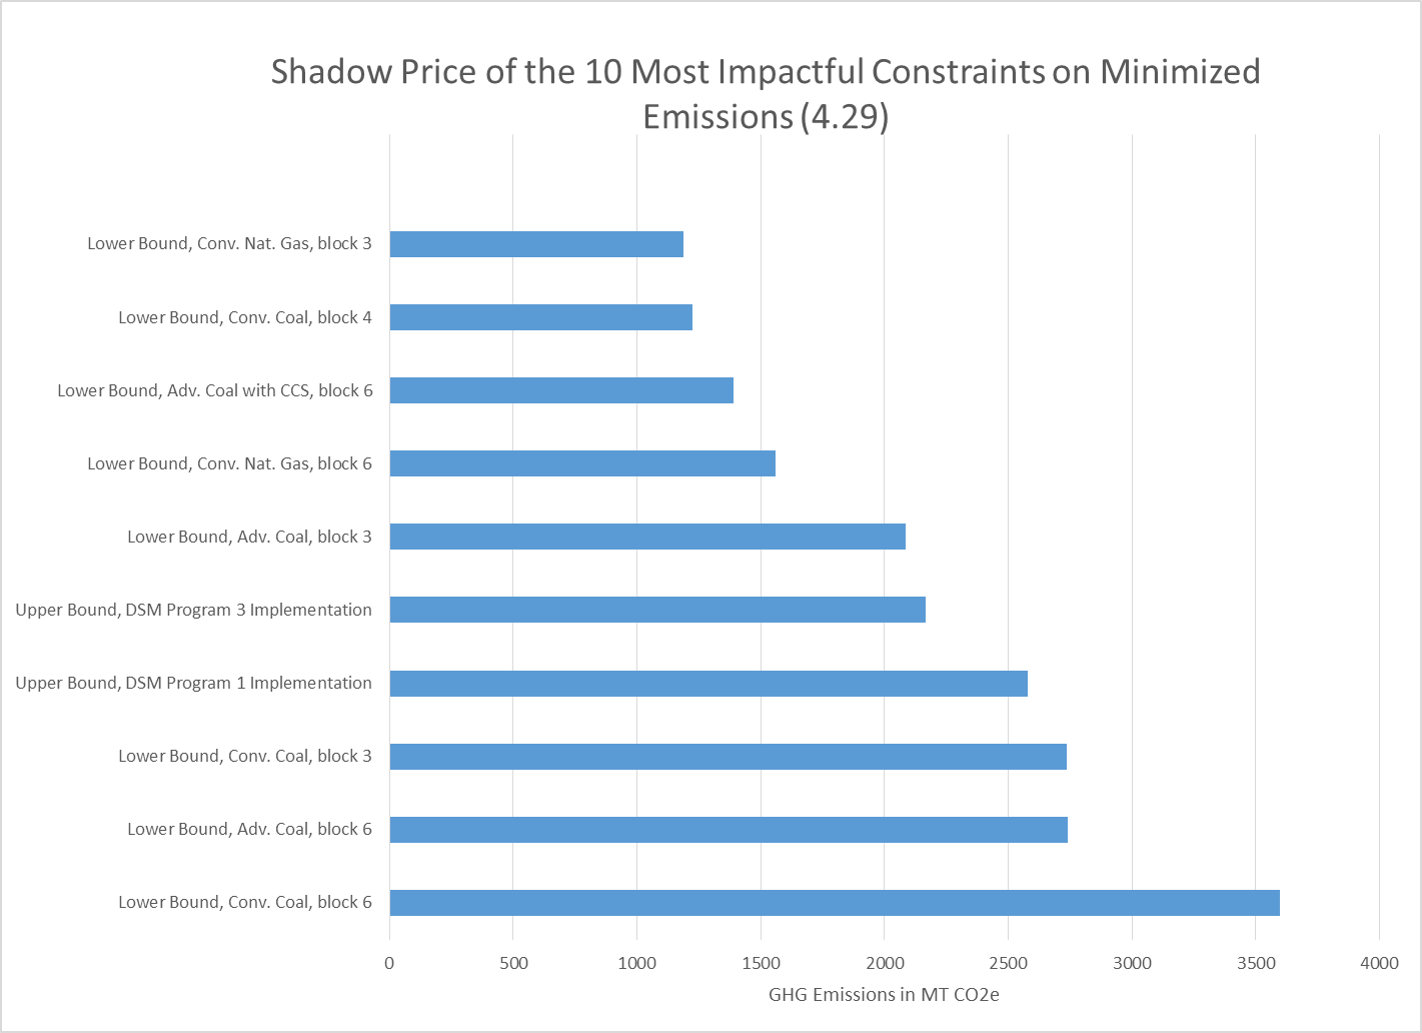
\includegraphics[width=\textwidth]{429_6_sensitivity}
		\caption{Shadow Prices of 10 Most Significant Constraints.}
		\end{figure}



%%%%%%%%%%%%%%%%%%%%%%%%%%%%%%%%%%%
\paragraph{4.30}
	A multi-objective optimization was performed between the minimum GWP and minimum expected cost objectives. The two objective functions, designated as $obj_1$ and $obj_2$ respectively, are combined into a single objective function. Both are multiplied by its own scaling factor, $\xi$, which brings them into the same order of magnitude based on the minimum solution for each. The parameter $\theta$ is used to weight the objectives; $\theta$ varies from zero to one, and the other factor is weighted by $1-\theta$. A step size of 0.001 was used (1000 runs). The single objective is described as follows: 

	\begin{align*}
		min \ \xi_1 \theta obj_1  + \xi_2 (1-\theta) obj_2 
	\end{align*}
	
	where:
	\begin{itemize}
		\item $\theta \in [0, 1]$: weighting/preference parameter between two objectives.
		\item $\xi_1, \xi_2$: scaling factor to bring $obj_1$ and $obj_2$, respectively, to $10^0$ magnitude
	\end{itemize}

	A Pareto frontier may be established by plotting the resultant values for each $\theta$. The values that make up the bottom edge of the frontier are Pareto efficient - i.e., at any point on the frontier, a reduction in cost requires an increase in GWP, or vice versa. Figure 7 presents the resultant Pareto frontier, with $\theta$ values expressed along a color gradient.
	
	\begin{figure}
		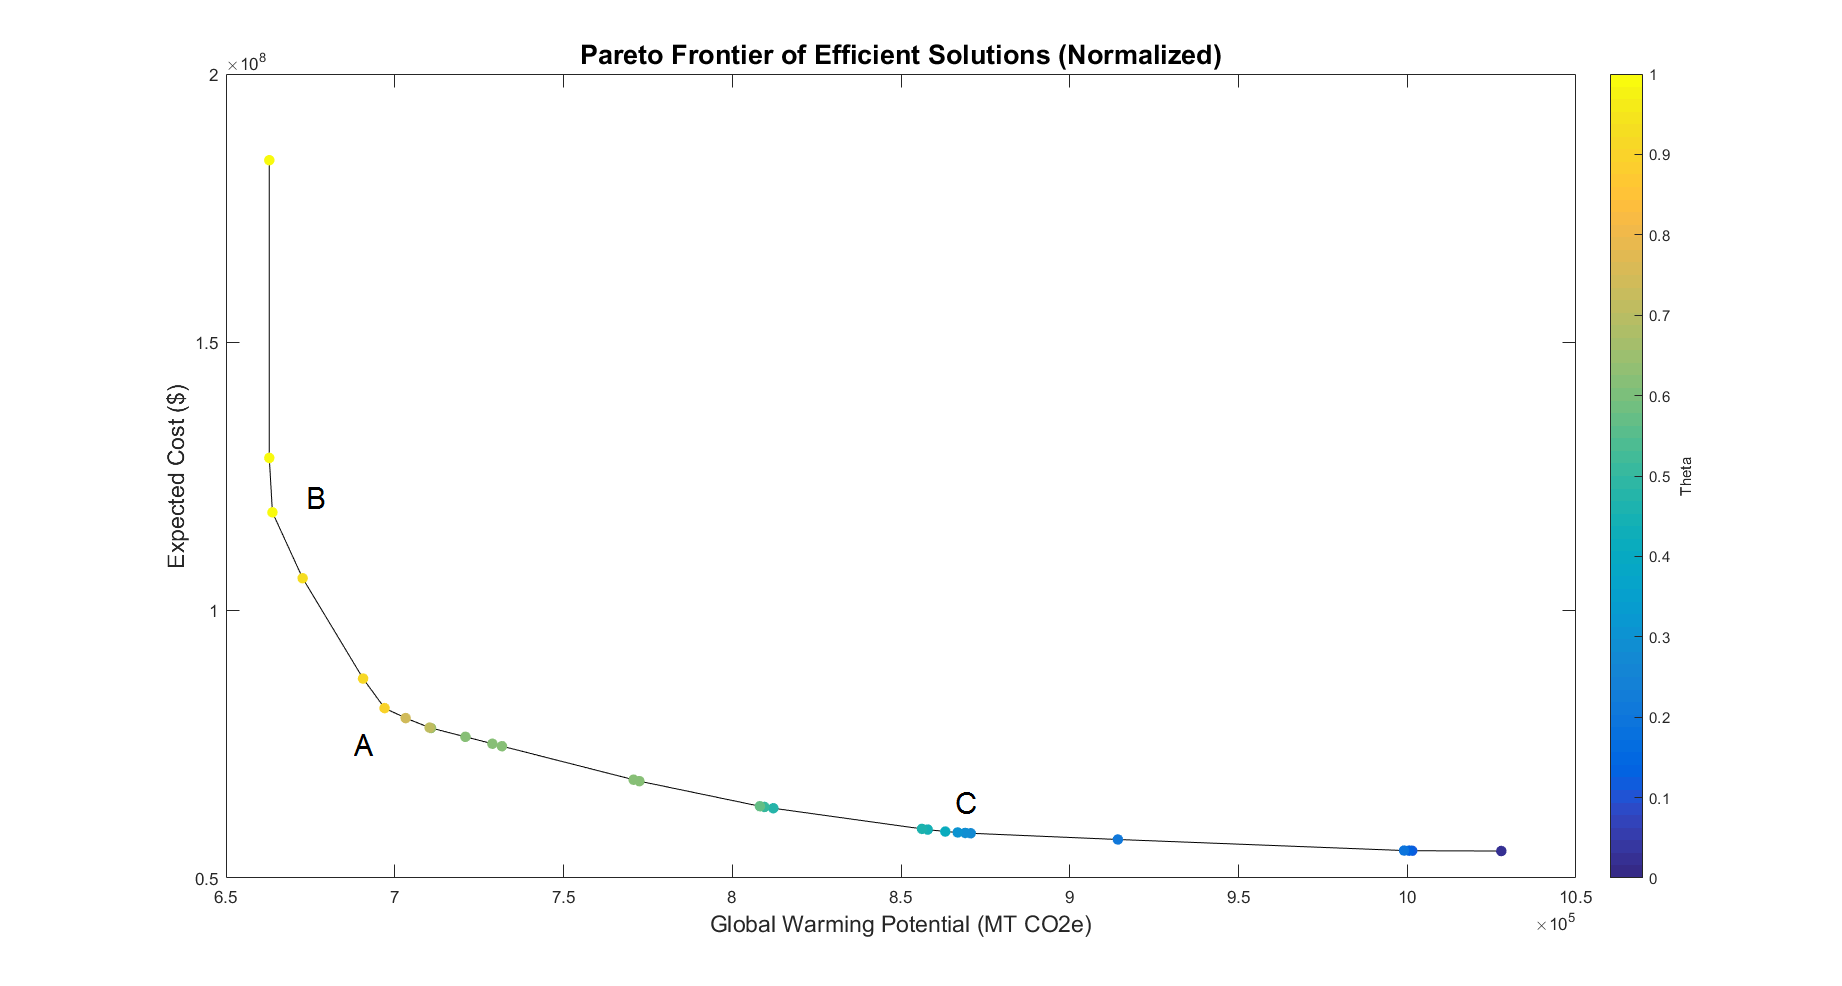
\includegraphics[width=\textwidth]{430_7_pareto_frontier}
		\caption{Generation in each load block per plant.}
	\end{figure}

	Points labeled A, B, and C in Figure 7 indicate kink points were a number of solutions are grouped, and a change in slope of the function is apparent. Point B is a solution that heavily weights minimizing GWP, while Point C is a solution that heavily weights minimum cost. Point A is a point that balances the two objectives and appears closest to the origin. It still weights GWP more heavily, as it occurs at $\theta \approx 0.8$. We select a median $x$ from the cluster around Point A and compare with the two previous solutions, as presented in Table 4.30a. 
	
	Compared to the minimum cost solution, this median result had an expected cost that was 48\% greater and a cost variance 66\% greater, with a GWP 32\% lesser. Compared to the minimum GWP solution, this median result had an expected cost that was 56\% lesser and a cost variance 58\% lesser, with a 5\% increase in GWP. 
	
	As the median result illustrates, minimizing either expected cost or GHG causes a spike in the other, with cost variance typically moving with expected cost. Additionally, since this median result selected was a point on the Pareto frontier close to the origin, it appears that expected cost is a more sensitive metric than GWP, as it increased about 10 times as much as GWP did. This is evident as well in Figure 5 when comparing the slope between AB and AC. 


%%%%%%%%%%%%%%%%%%%%%%%%%%%%%%%%%%%%
\paragraph{4.31}
	An emissions cap constraint may be added to the minimum expected cost optimization problem by adding the objective function of the minimum GWP problem to inequality constraints $A$ and $b$, as follows:
	
	\begin{align*}
		min \ 0.001 \sum_{i=1}^{I} \sum_{t=1}^{T} g_i n_t x_{it} \leq \gamma
	\end{align*}
	
	where $\gamma$ is the emissions cap in MT CO2e. If $\gamma$ is set to the minimum GWP value achieved in Part 4.29, this effectively forces the minimum GWP solution. However, we varied the cap around the GWP solution, from 500,000 MT to 1.1 million MT, and ran an optimization for each value. The results are presented in the plot in Figure 8.
	
	\begin{figure}
		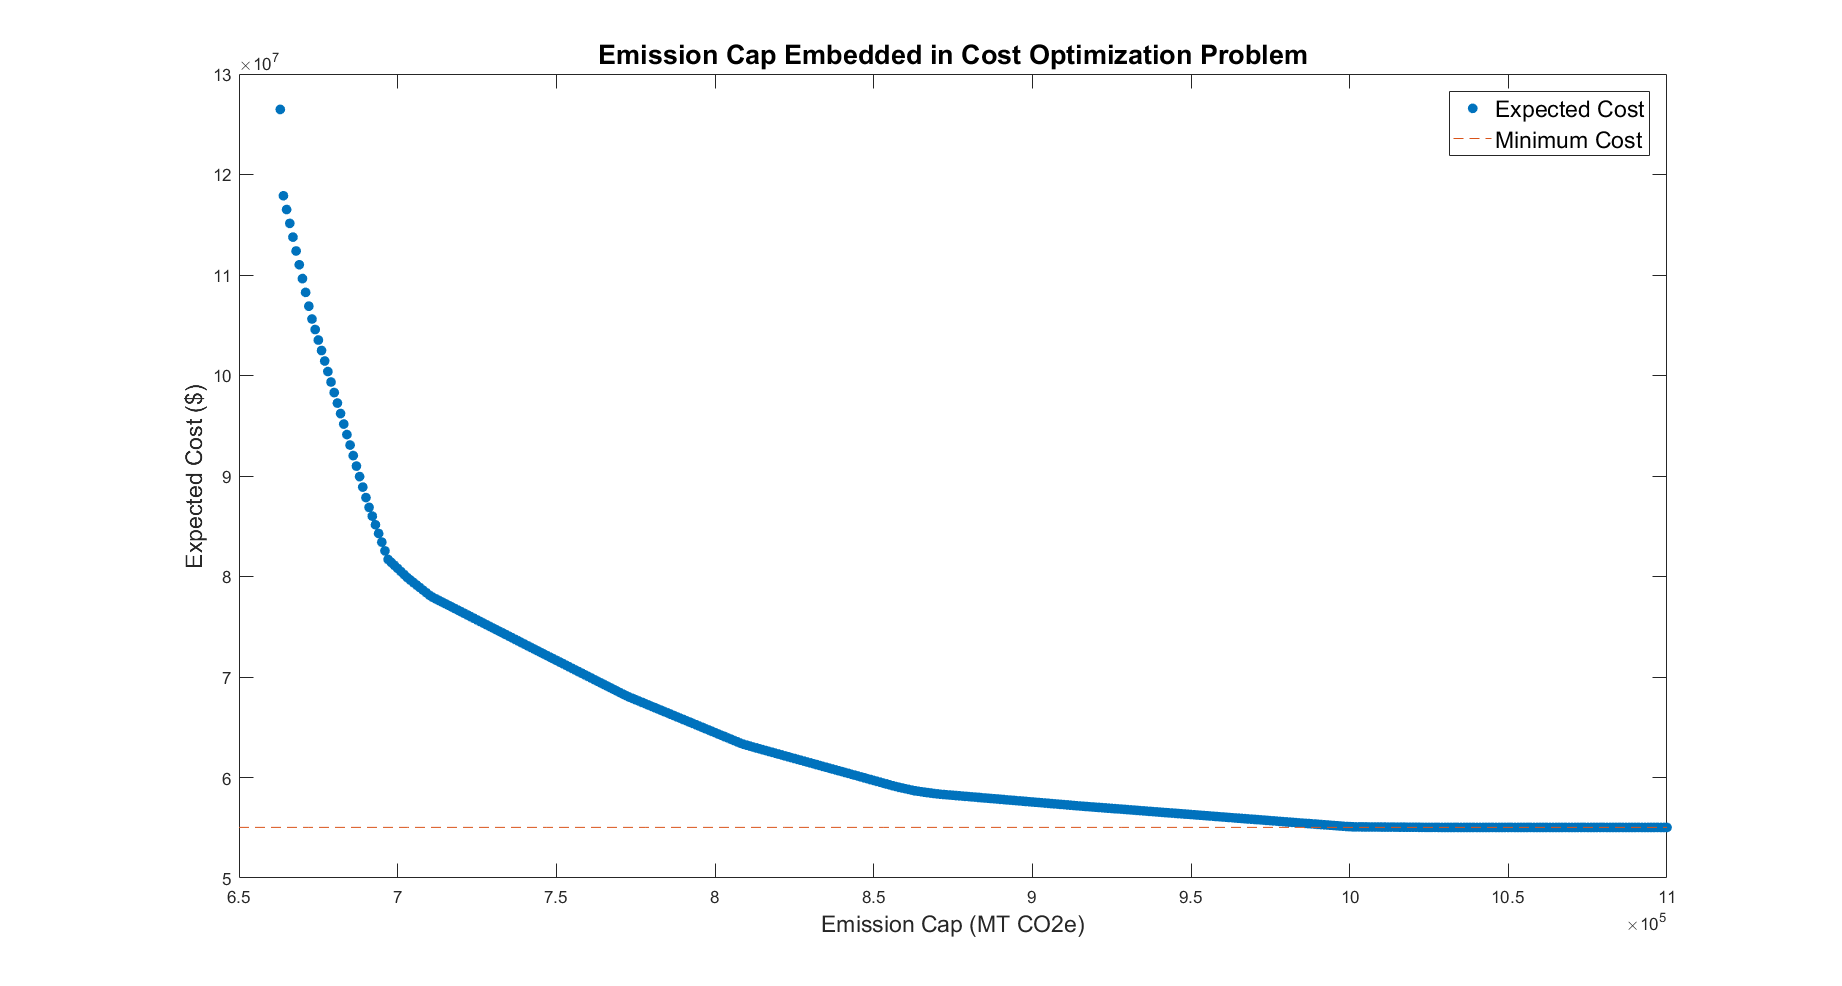
\includegraphics[width=\textwidth]{431_8_cap_figure_plot}
		\caption{Minimum Cost Result with Varying Emissions Cap.}
	\end{figure}

	The horizontal line is plotted at the minimum cost solution of \$55 million. This minimum value is reached at a cap value of 1.028 million MT, meaning that below this value, the cap is influencing the minimum cost solution by increasing the cost. As expected, for the cap values set below the minimum GWP solution, the linear program was not valid; providing electricity sufficient to meet demand is not possible below that limit. There are a number of kinks in the curve where there is a slope change.


%%%%%%%%%%%%%%%%%%%%%%%%%%%%%%%%%%%%
\paragraph{4.32}
	Another regulatory approach to curbing emissions is a carbon tax applied to emissions in dollar per kilogram, formulated as $\tau$ in this problem. The tax may be added to the objective function of minimum expected cost problem by adding constants $g_i$ to the $x_{it}$ decision variables to include emissions, as follows:
	
	\begin{align*}
		min \sum_{t=1}^{T} \bigg\{ 
		\sum_{i=1}^{I} \big( n_t x_{it} (\bar{c}_i^v + \tau g_i) + 1000y_i \bar{c}_i^c \big)
		+ \sum_{k=1}^{K}  n_t \bar{c}_k^d z_k s_{kt}^{max}
		\bigg\}
	\end{align*}
	
	Constraints remain the same as in Part 4.28. We performed the minimum cost optimization problem with initial tax values ranging from \$0 to \$20 per kg of CO2e. We found that the latter was around an order of magnitude too high, and subsequently focused on values below \$1. Figure 9 presents a plot of the expected cost vs. tax, scaled to tax values of zero to \$0.50. As expected, it is not possible to set a tax that retains the minimum expected cost solution, which makes sense, as adding cost monotonically (though not linearly) increases the expected cost. 
	
	\begin{figure}
		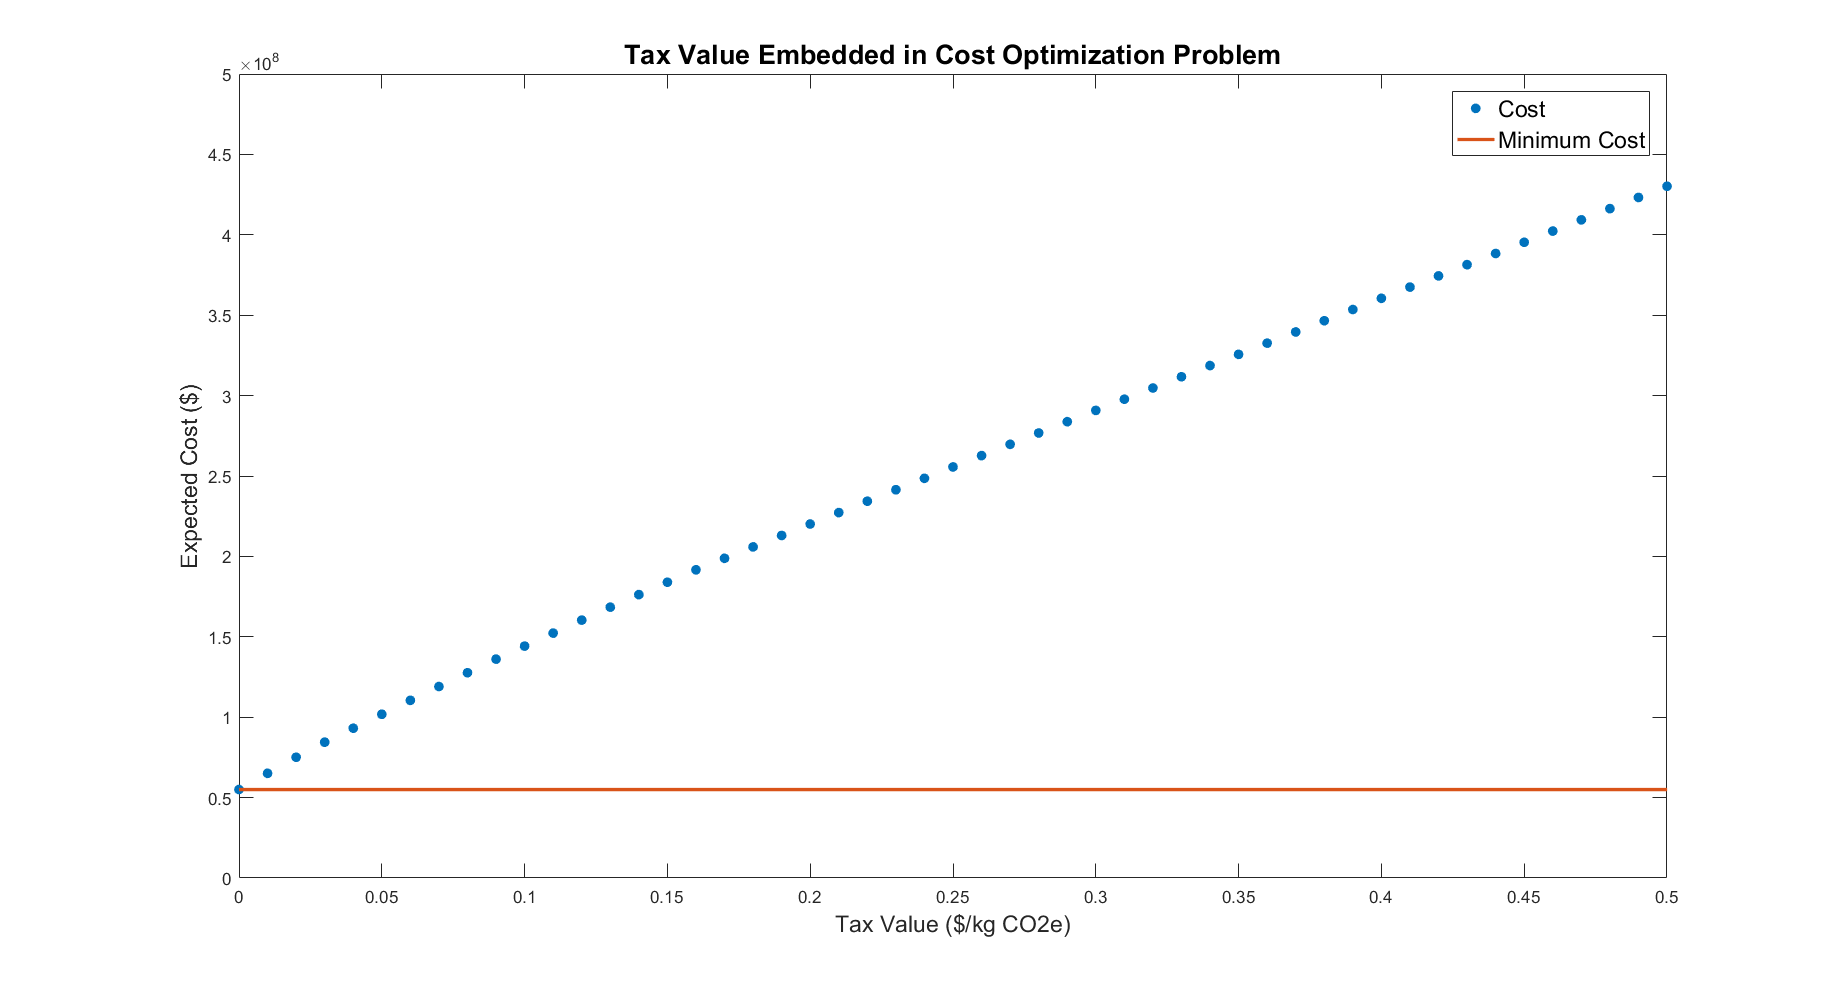
\includegraphics[width=\textwidth]{432_9_cost_vs_tax_zoomed}
		\caption{Expected cost vs. carbon tax.}
	\end{figure}
	
	Next, carbon taxes values were analyzed as an alternative to the emission cap. It is possible to identify a tax value that affects cost in a way such that the same emissions are achieved as in the minimum GWP problem; as the tax increase, the generation portfolio shifts towards renewables until emissions on parity with the minimum GWP problem are achieved, which is the lowest that emissions can be driven. This specific tax value is \$10.91/kg CO2e, as shown on Point A in Figure 10. However, GWP value that is just 0.14\% higher than minimum can be achieved at a much lower tax value of \$1.38/kg CO2e, which is indicated as Point B in Figure 10. Between \$1.38 and \$10.91, the values of GWP remain constant. Indeed, as shown in Figure 10, GWP is a step function as tax increases. This shows that a utility design can be flexible and shift around generation between sources even as taxes increase to maintain a certain GWP level. Moreover, the steps decrease rapidly over the initial values of the tax, from \$0 to \$0.20. It appears that adding even a small tax significantly affects the solution, and the effect levels off as the tax increases.
	
	\begin{figure}
		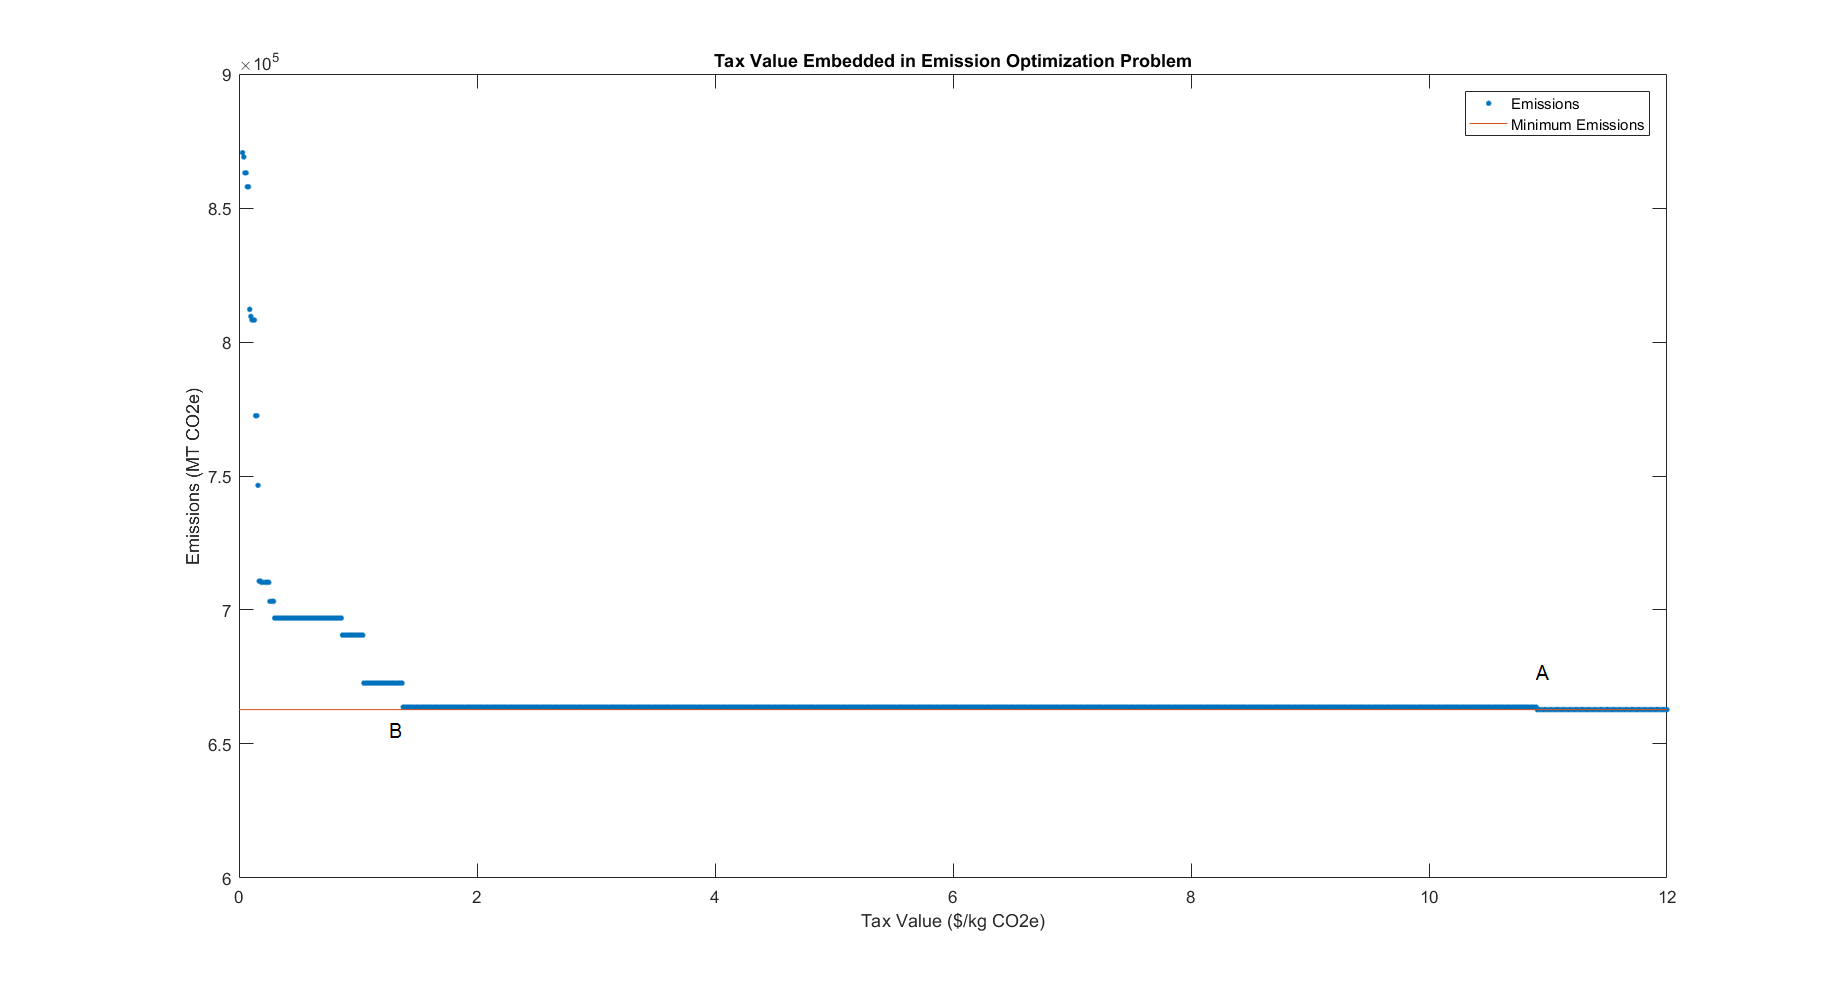
\includegraphics[width=\textwidth]{432_10_tax_vs_minemissions}
		\caption{Emissions vs. Carbon Tax}
	\end{figure}
	
	We investigated carbon taxes that have been implemented in practice or proposed in other Anglo-Saxon countries to provide a comparison point for our result. Generally, the enacted taxes are in the 1-10 cent range per kg, meaning the \$1.38/kg result is one to two orders of magnitude higher than actual carbon taxes. Select carbon taxes are summarized below:
	
	\begin{itemize}
		\item Washington State: ballot measure I-732 was defeated by voters in November 2016. The tax would have started at \$0.015/kg in 2017 and increased to \$0.10/kg [1].
		\item British Columbia: tax enacted in 2008 at CAD 10/MT, with a current value of CAD 30/MT [2]. This corresponds to USD \$0.023/kg.
		\item Canada: new carbon tax policy announced in November 2016. Tax reaches a final value of CAD 50/MT in 2022, or \$0.038/kg [3].
		\item Australia: tax enacted in 2012 and repealed in 2014. Final price was USD \$0.02/kg [4].
	\end{itemize}



%%%%%%%%%%%%%%%%%%%%%%%%%%%%%%%%%%%%
\paragraph{4.33}
	A third optimization problem is solved to find the minimum cost variance, as controlling variability and uncertainty is a crucial component in system design. 
	
	\subparagraph{Setup}
		The objective function is based on that of the minimum cost problem in Part 4.28, but in squared terms to work with cost variance. 
	
	\begin{align*}
		min \sum_{t=1}^{T} \bigg\{ 
		\sum_{i=1}^{I} \big( n_t^2 x_{it}^2 (\sigma_i^v)^2 + 1000^2 y_i^2 (\sigma_i^c)^2 \big)
		+ \sum_{k=1}^{K}  n_t^2 z_k^2 (s_{kt}^{max})^2 (\sigma_k^d)^2 
		\bigg\}
	\end{align*}
	
	where:
	\begin{itemize}
		\item $\sigma_i^v$: standard deviation of variable cost for plant $i$ in \$/MWh, $\forall i$
		\item $\sigma_i^c$: standard deviation of capital cost for new plant $i$ in \$/kw, $i \in [5,8]$
		\item $\sigma_k^d$: standard deviation of cost for DSM program $k$ in \$/MWh, $\forall k$
	\end{itemize}
	
	This problem is a non-linear program, and was solved using MATLAB's \texttt{quadprog} solver with the interior point algorithm. This required formulating the problem as follows:
	
	\begin{align*}
		\underset{x}{\min} \ \frac{1}{2} x^T H x + f^T x\ 
		s.t. \Bigg\{ \substack{
		A \cdot x  \leq b \\
		Aeq \cdot x \leq beq \\
		lb \leq x \leq ub}
	\end{align*}
	
	$H$ is a square matrix of dimension 61, for each decision variable. $H$ incorporates both the covariance matrix and off-diagonal terms with constant values from the minimum cost objective function, as follows:
	
	\begin{align*}
		H_{61,61} &= H_0^T \Sigma H_0 \\
	\end{align*}
		where:
	\begin{align*}
		\Sigma_{16,16} = \begin{bmatrix} 
			(\sigma_1^v)^2 & 0 & \cdots & \cdots & \cdots & \cdots & \cdots & \cdots & \cdots & 0 \\
			0 & (\sigma_2^v)^2 & 0 & \cdots & \cdots & \cdots & \cdots & \cdots & \cdots & 0\\
			\vdots & \cdots & \ddots & \cdots & \cdots & \cdots & \cdots & \cdots & \cdots & \vdots \\
			0 & \cdots & \cdots & (\sigma_9^v)^2 & \cdots & \cdots & \cdots & \cdots & \cdots & 0\\
			0 & \cdots & \cdots & \cdots & (\sigma_5^c)^2 & \cdots & \cdots & \cdots & \cdots & 0\\
			\vdots & \cdots & \cdots & \cdots & \cdots & \ddots & \cdots & \cdots & \cdots & 0\\
			0 & \cdots & \cdots & \cdots & \cdots & \cdots & (\sigma_8^c)^2 & \cdots & \cdots & 0 \\
			0 & \cdots & \cdots & \cdots & \cdots & \cdots & \cdots & (\sigma_1^d)^2 & \cdots & 0 \\
			0 & \cdots & \cdots & \cdots & \cdots & \cdots & \cdots & \cdots & (\sigma_2^d)^2 & 0 \\
			0 & \cdots & \cdots & \cdots & \cdots & \cdots & \cdots & \cdots & \cdots & (\sigma_3^d)^2\\
			\end{bmatrix} \end{align*}
	\begin{align*}
		H_{0 \ (16,61)} = \begin{bmatrix}
				X_{0 \ (9,54)} & 0 & 0 \\
				0 & Y_{0 \ (4,4)} & 0 \\
				0 & 0 & Z_{0 \ (3,3)} \\ 
			\end{bmatrix}
	\end{align*}

	$\Sigma$ is the covariance matrix. Decision variables are assumed to be statistically independent, so off-diagonal elements are all zero (no covariances). $X_0$, $Y_0$, and $Z_0$ are the coefficient matrices for $x_{it}$, $y_i$, and $z_k$, respectively, with coefficients defined in the minimum cost optimization problem $f$ vector.
	
	\subparagraph{Results}
	Variance generally is reduced through variety and spreading of costs and generation. This is reflected in the solution for the minimum variance solution. All new generation sources are built, with sizes roughly corresponding to the inverse of its capital cost variance; i.e., the lowest-variance new generation source, advanced CC natural gas, was built at the largest capacity, and the highest-variance new source, solar, was built at the smallest capacity. 
	
	All generation sources were used in the heavier load blocks. In the lighter load blocks, more generation sources were used as well compared to the minimum cost and minimum GWP solutions. All three DSM programs were implemented as well, with program 1 at about 32\% and the others at their full rates; it seems that cost variance associated with DSM is less significant than the variance reduction achieved through reduction in power requirements. The solution is presented in Table 4.33a.
	
	The expected cost for this solution is \$8.4064e+07, or about \textbf{\$84 million}, or about 53\% more than the minimum expected cost. GWP of this solution is 1.0716e+06 MT, or about \textbf{1.1 million MT} CO2e, which is about 62\% more than than the minimum GWP. Finally, the minimum variance found is \$2.0035e+13, which gives a cost standard deviation of \$4.4760e+06, or about \textbf{\$4.5 million}. This is a significant reduction compared to the minimum expected cost solution's standard deviation of \$6.2 million. 
	
	

%%%%%%%%%%%%%%%%%%%%%%%%%%%%%%%%%%%%
\paragraph{4.34}

	A multi-objective minimization was performed between the minimum expected cost and minimum cost variance objectives. The same scaling factor $\xi$ and weighting parameter $\theta$ approach was used as in Part 4.30. The single objective is described as follows, where $obj_2$ and $obj_3$ are the minimum cost and mininum variance objectives, respectively. A step size of 0.01 was used.

	\begin{align*}
		min \  \xi_2 \theta \ obj_2  + \xi_3 (1-\theta) \ obj_3 
	\end{align*}
	
	Since $obj_3$ is quadratic, it was necessary to formulate $obj_2$ as a quadratic program. This was achieved by simply setting its $H$ matrix to be a square zeros matrix, in accordance with the formulation described in Part 4.33. 
	
	The resultant Pareto frontier is presented in Figure 11. Point A represents an apparent kink point with a cluster of solutions ($0.32 \leq \theta \leq 0.47$) and an apparent change in slope. Moreover, this point appears close to the origin. We select a median solution from the cluster with $\theta = 0.39$, which slightly favors variance minimization.
	
	For this median solution, the expected cost is \$6.2648e+07, or about \textbf{\$63 million}, which is a 14\% increase over the minimum expected cost. The GWP impact is 1.2066e+06 MT, or about \textbf{1.2 million MT}, which is 82\% higher than the minimum GWP solution. The cost variance is \$2.3553e+13, corresponding to a standard deviation of \$4.8531e+06, or about \textbf{\$4.9 million}. This represents an 8\% increase over the minimum cost standard deviation.
	
	From the results of the two multi-objective optimizations, minimization of two of the three objectives is at the expense of the third objective. Expected cost and cost variance appear to move together more closely.
	
	\begin{figure}
		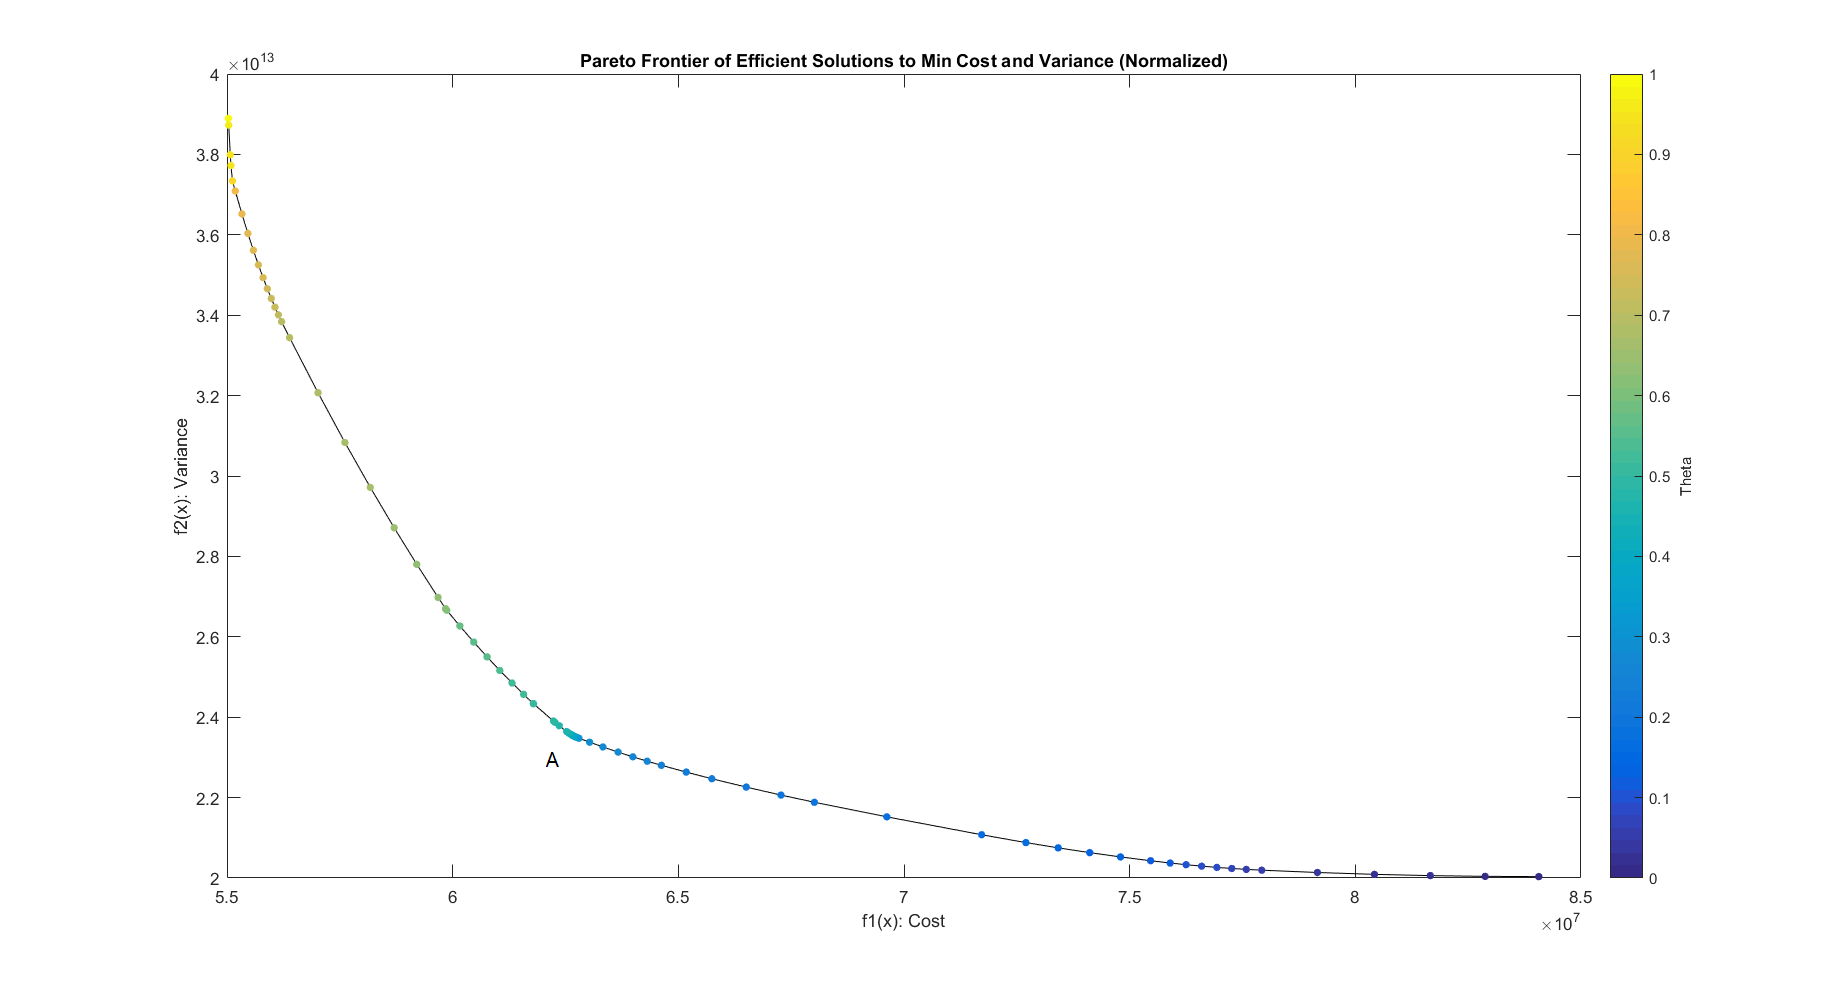
\includegraphics[width=\textwidth]{434_11_cost_var_pareto}
		\caption{Pareto frontier for expected cost vs. variance optimization}
	\end{figure}
	


%%%%%%%%%%%%%%%%%%%%%%%%%%%%%%%%%%%%
\paragraph{4.35}
	In this section, we propose an overall design for the utility.
	
	\subparagraph{Prior Findings}
		Several general findings from the prior analyses were used to help inform the design process:
	
	\begin{itemize}
		\item Minimizing expected costs favors existing generation and new fossil sources.
		\item Minimizing GWP favors nuclear, hydroelectric, and new wind and solar sources.
		\item Minimizing variance encourages portfolio diversity, both in terms of new construction and energy provision in all load blocks.
		\item While in a strict sense, expected cost and variance are different objectives that have trade-offs, these two objectives move more closely together comparead to GWP.
		\item Minimal GWP appears more easily preserved than minimal cost in multi-objective optimizations, as median solutions that are visually close to the origin more heavily weight GWP.
	\end{itemize}

	The minimum values of the three objectives are used as baselines for our solution:
	
	\begin{itemize}
		\item Expected cost: \$5.5031E07
		\item GWP: 6.6283E05 MT
		\item Variance: $\$^2$ 2.0035E13
	\end{itemize}
	
	\subparagraph{Approach}
		We conduct a triple-objective optimization between the three objectives to calculate the tradeoffs between the three solutions. We observe the effect on the third objective when comparing two objectives. Next, we use a screening approach to reduce the number of eligible solutions produced by the triple-objective optimization. This approach finds solutions within a tolerance range of the minimum solutions for all three objectives. 
		
		This subset is analyzed on two additional criteria - minimum new construction (total new MW) and minimum use of intermittent sources (wind, solar, hydroelectric) - to select a proposed design. These criteria are essentially a qualitative approach to further reducing variance. 
		
		We selected the former because we assume the utility faces additional flow-down costs from each plant construction that are not directly captured in the direct capital and variable costs, such as opportunity costs for capital and labor, and added complexity in system management. 
		
		We selected the latter because of the inherent uncertainty in intermittent generation sources. While intermittency should be captured in the unplanned outage rate $o^u$, and we analyze one such situation in Part 4.37, we again assume there may be indirect effects associated with renewable sources. Hydroelectric power requires maintaining a presence in remote, mountainous areas, as well as various added regulatory burdens associated with surface water protection, wildlife management, etc. Management of large dams also burdensome due to the n-sigma risk associated with catastrophic failure that does not exist for other generation sources. Finally, hydroelectric facilities are generally older, and new capacity cannot be built. Regarding wind and solar, both are large land footprint endeavors, and we assume potential additional risks and regulatory burden associated with dealing with multiple landowners and maintaining a larger distribution infrastructure. Since we are already screening solutions within a tolerance limit of the optimal GWP solution, we are comfortable with picking a relatively non-renewable solution from that subset.
		
		
	\subparagraph{Triple-Objective Optimization}
		A triple-objective optimization between expected cost, GWP, and variance was performed. The same scaling factor $\xi$ and weighting parameter $\theta$ approach was used. A second weighting parameter $\phi$ is introduced, such that $1-\theta-\phi$ is the weight of the third objective and the sum of all three is less than 1. The combined objective function is described as follows, where $obj_1$, $obj_2$, and $obj_3$ are the complete minimum cost, minimum GWP, and mininum variance objective functions, respectively:
		
		\begin{align*}
		min \  \xi_1 \theta \ obj_1  + \xi_2 \phi \ obj_2  + \xi_3 (1-\theta-\phi) \ obj_3 
		\end{align*}
		
		A step size of 0.01 was used for the scaling factors. This produced 5,151 eligible scaling factor combinations, which is how many optimizations were run. As was the case in Part 4.34, $obj_1$ and $obj_2$ were written in \texttt{quadprog} format by setting their H matrices to zeros.
		
		Figure 11 shows a 3D plot containing the resultant solutions from the triple-objective optimization. The result appears to be a curved surface with edges that curl upwards - for eaxmple, the edge that minimizes cost and GWP curves upwards, indicating the higher variances associated with pursuing either minimum objective. Balanced solutions occur centrally and towards the bottom, while there is a trailing ``handle'' of exponentially-increasing variance for the bottom end of the minimum GWP solutions.
		
		\begin{figure}
			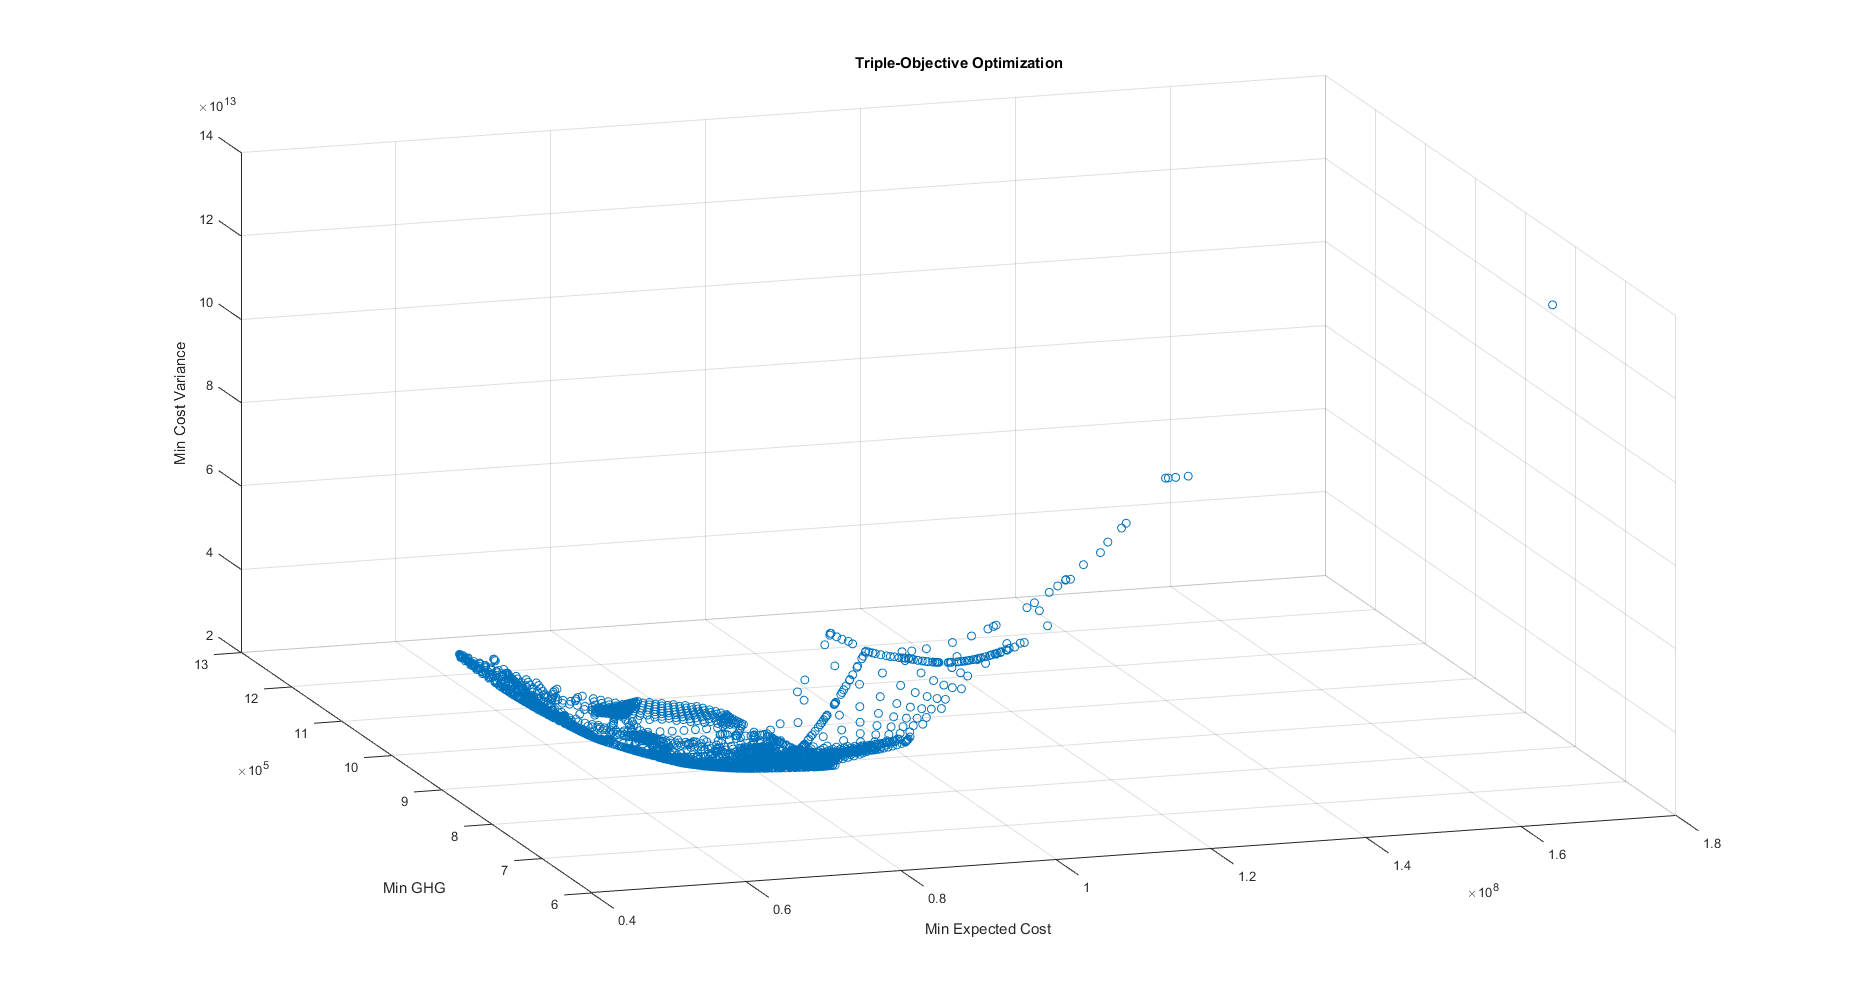
\includegraphics[width=\textwidth]{435_12_tripleobj}
			\caption{Triple-objective optimization results}
		\end{figure}
	
		Figures 12 to 14 present 2D plots of two objectives at a time, with the magnitudes of the third objective indicated by color. Smaller values of the third objective are indicated by darker colors. These figures further illustrate that pursuit of two objectives is at the expense of the third, and that balanced solutions do not occur at any of the Pareto frontiers for just two objectives.
		
		\begin{figure}
			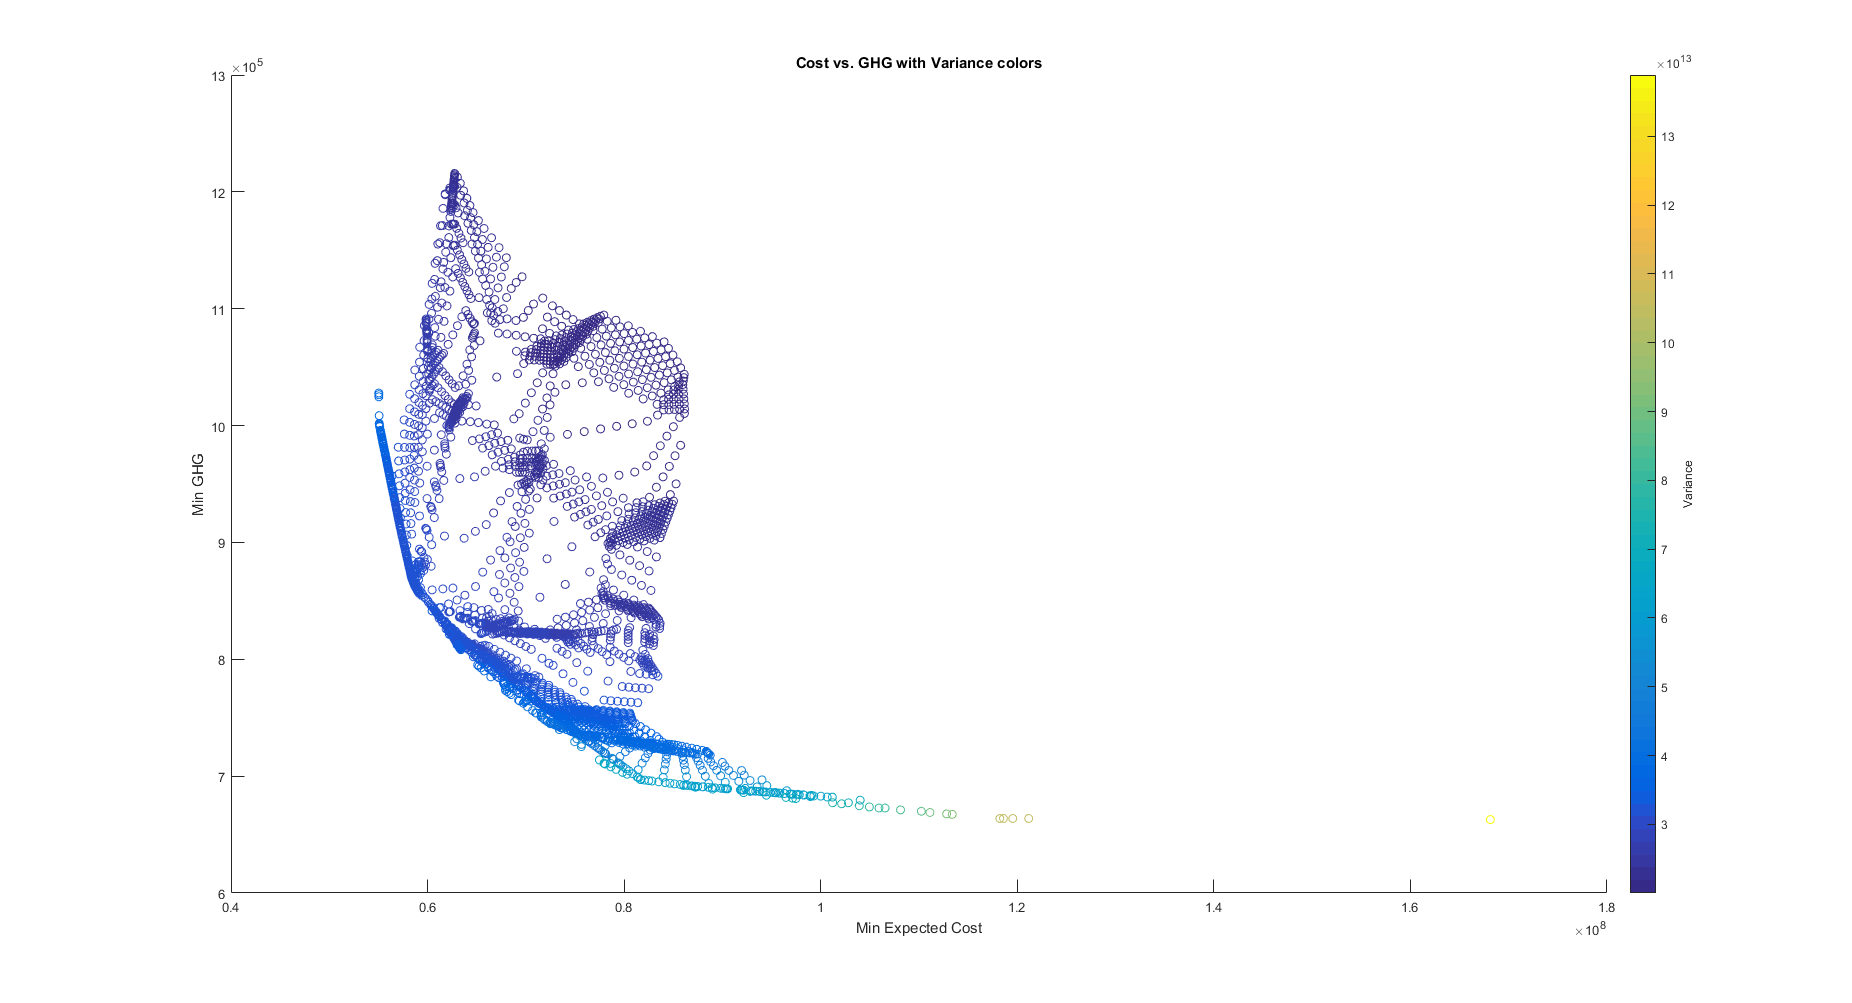
\includegraphics[width=\textwidth]{435_13_costghg}
			\caption{Cost vs. GWP with Variance Magnitude in Color}
		\end{figure}
		
		\begin{figure}
			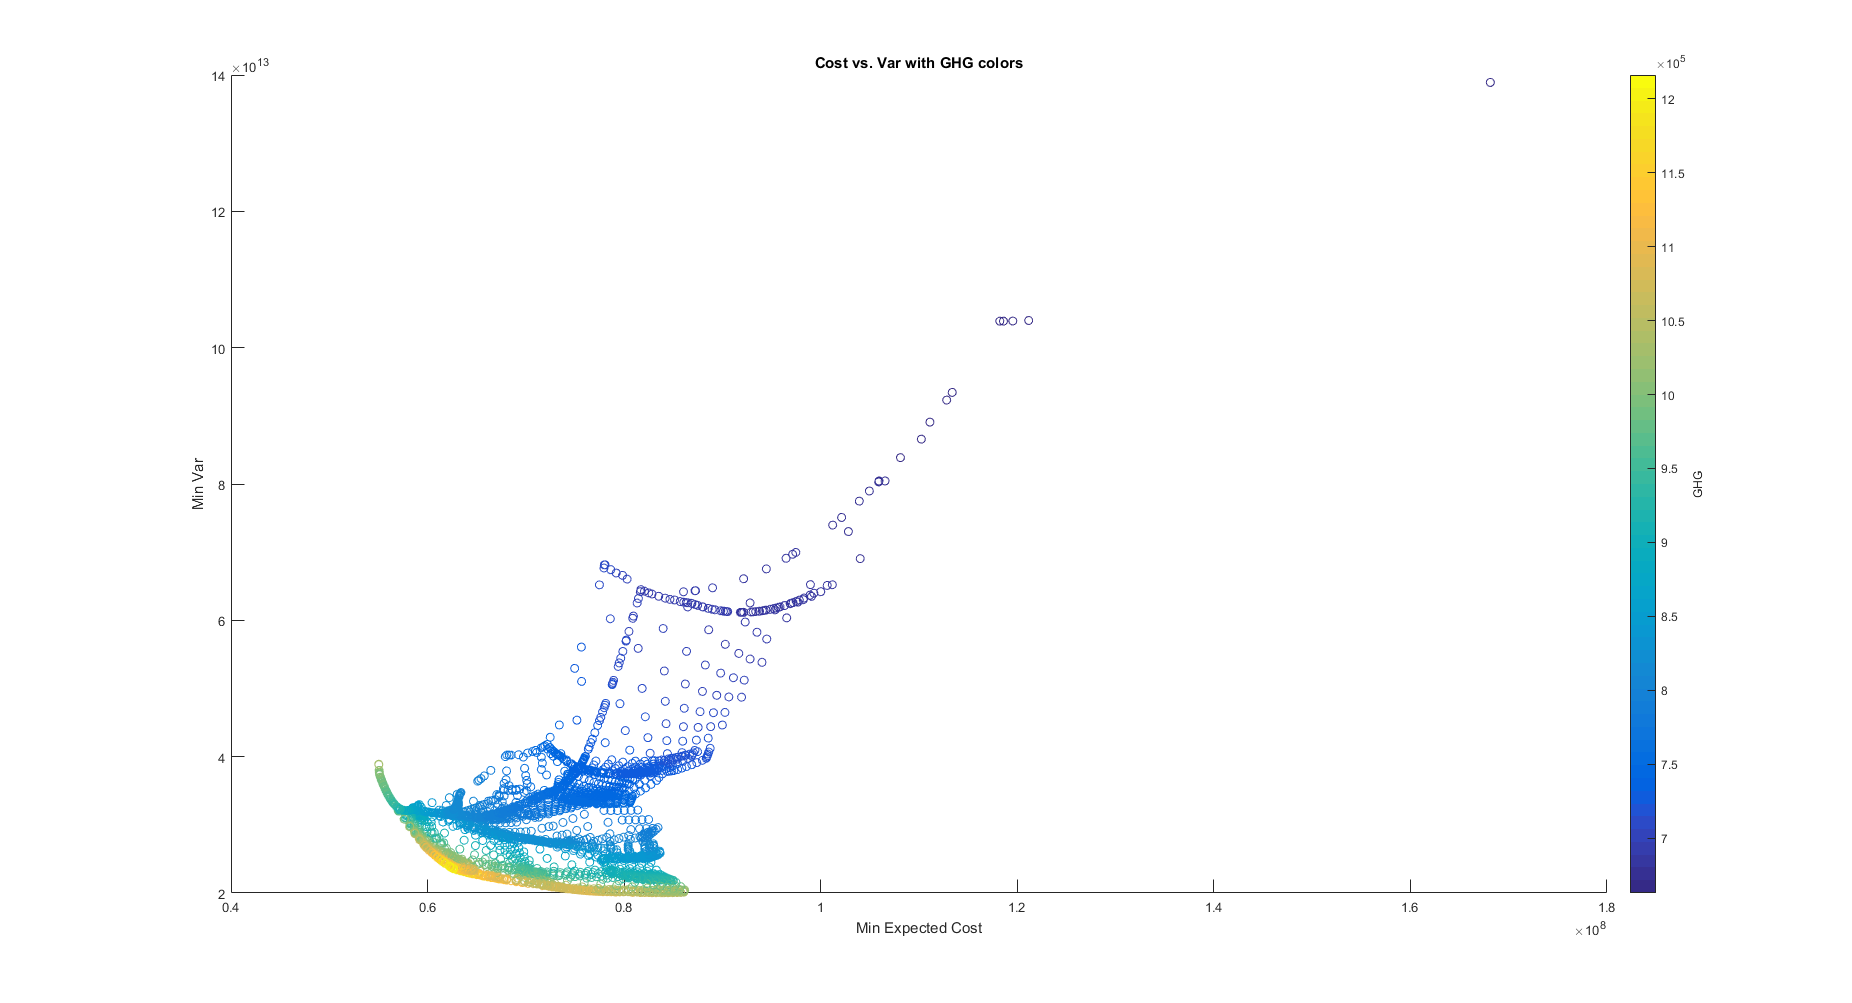
\includegraphics[width=\textwidth]{435_14_costvar}
			\caption{Cost vs. Variance with GWP Magnitude in Color }
		\end{figure}
		
		\begin{figure}
			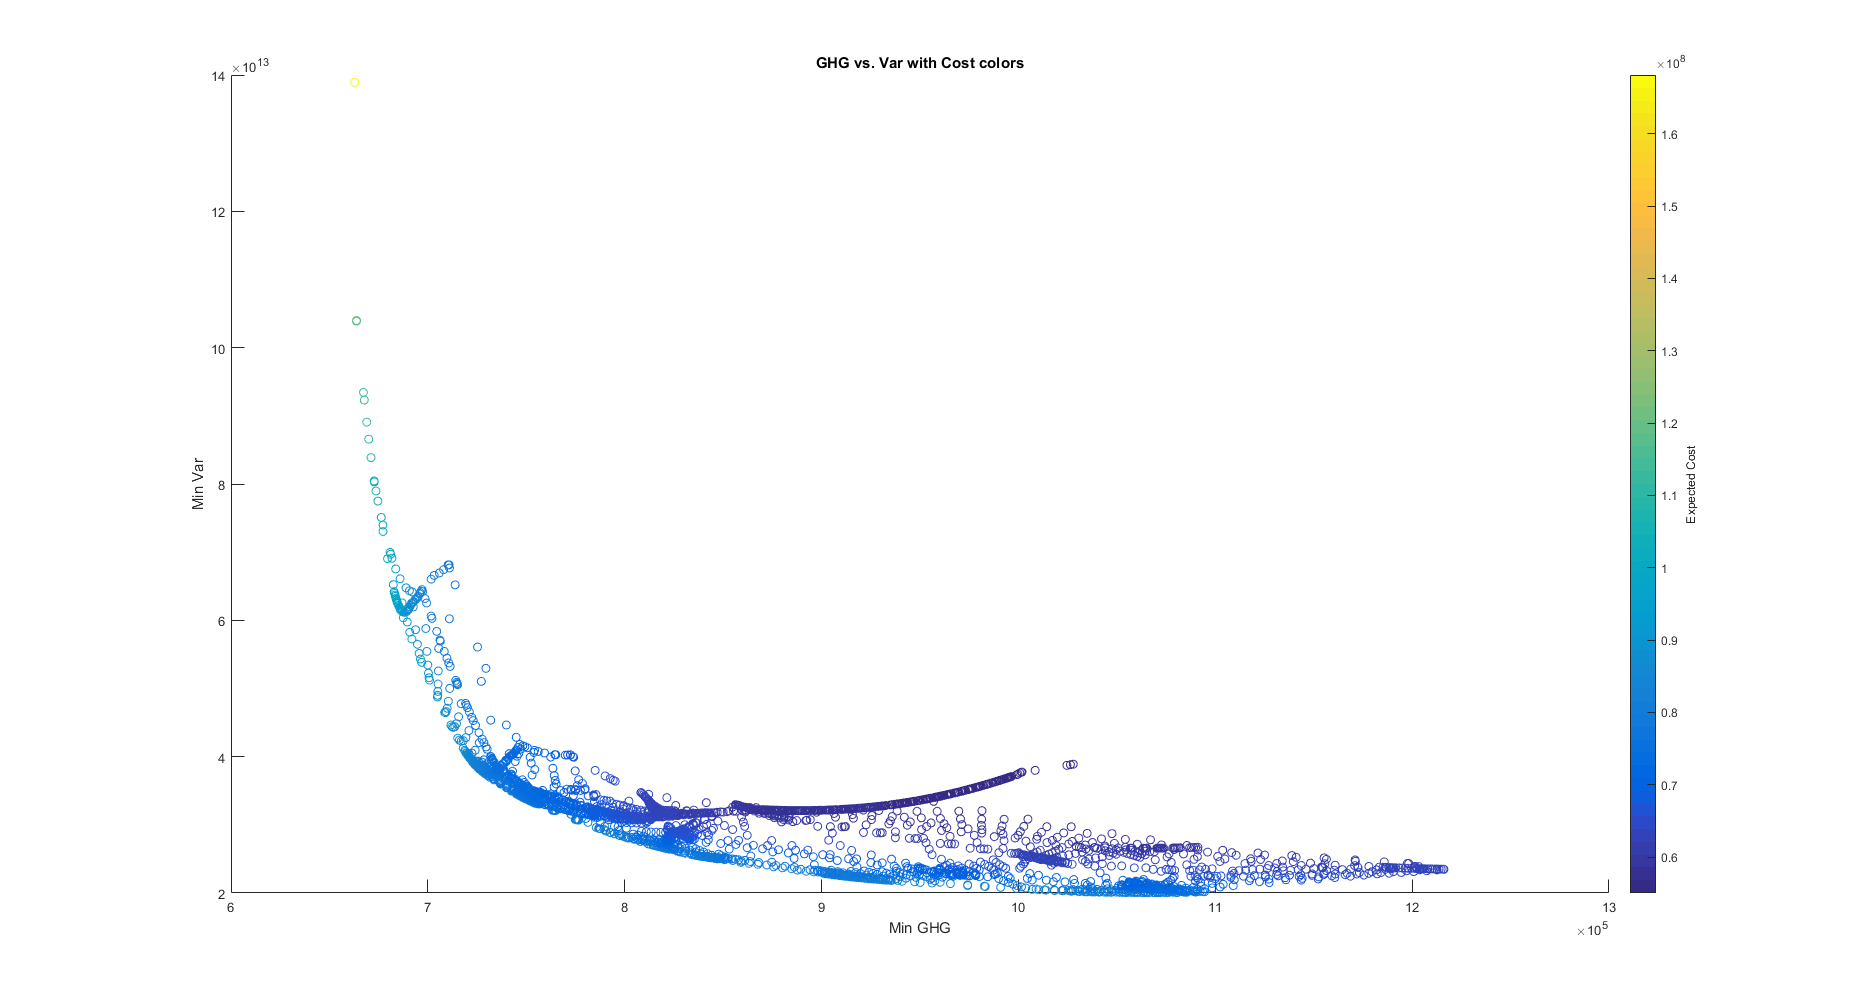
\includegraphics[width=\textwidth]{435_15_ghgvar}
			\caption{GWP vs. Variance with Cost Magnitude in Color}
		\end{figure}
		
		
		Based on these results, we applied the balanced screening approach discussed above. We do not prefer any of the three objectives over the others.
		
	\subparagraph{Screening Solutions}
		We calculated the cost, GWP, and variance of each of the 5,151 solutions found in the multi-objective optimization, and screened the solutions with a tolerance percentage above each of the minimum results. Solutions passed the screening if they were within a specified tolerance percentage of all three minimums. The percentage was slowly incremented until a set of passing solutions was found. At 35\% above the minimum, a set of 18 solutions passed. These solutions were then analyzed for total new construction MW and total reliance on intermittent sources, as defined above.
		
		All 18 solutions constructed all 4 eligible new plants. This result is sensible since it is consistent with a minimum variance objective, and with the GWP objective to a lesser extent. The total new construction size and renewable reliance were plotted and is shown on Figure 16.
		
		\begin{figure}
			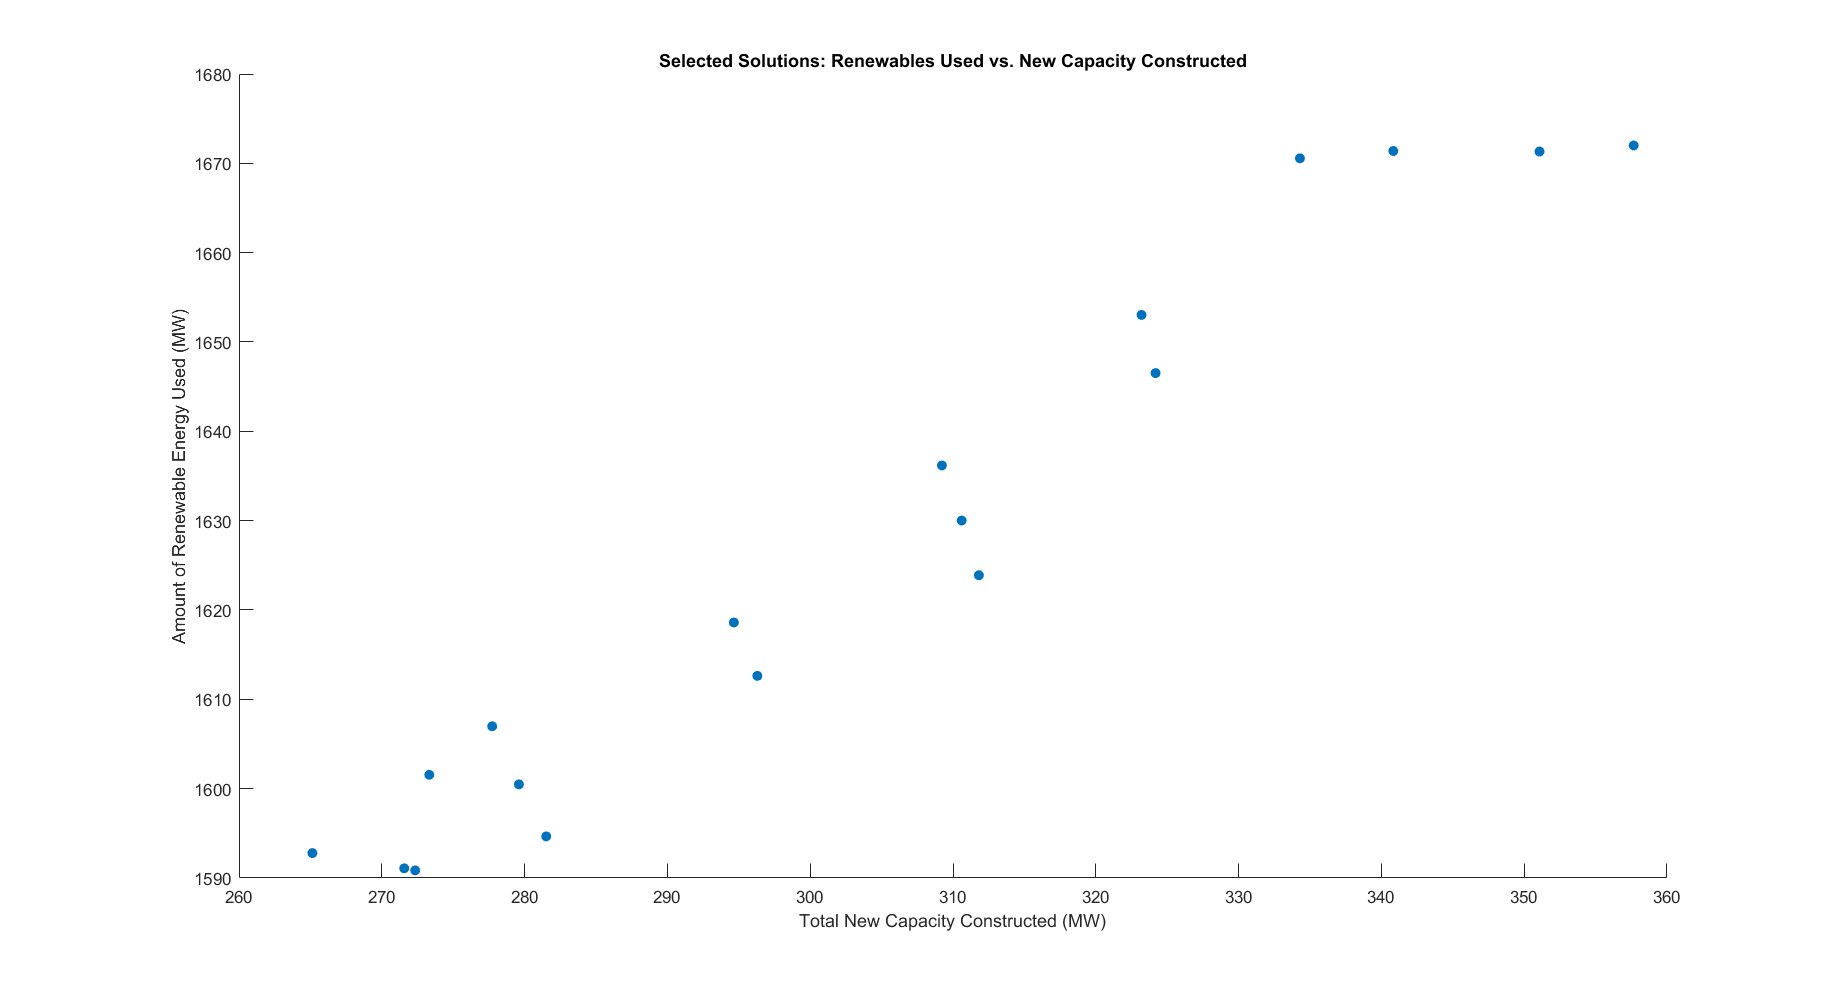
\includegraphics[width=\textwidth]{435_16_renMW_vs_newMW}
			\caption{Renewables Reliance vs. New Constructions - Screened Solutions}
		\end{figure} 
		
		A linear trend is apparent. This makes sense because the wind and solar are new constructions, so any use of those two requires new construction, and hydropower utilization is generally consistent between solutions, since it is a baseload source. We select the bottom left solution, which is lowest new capacity constructed option and the 3rd-lowest renewables reliance option. This solution is shown in Table 4.35a.
		
		For two of the new plant constructions, the results for advanced coal with CCS and solar are fractional, which is an artifact of optimization. In order to set these values and their corresponding $x_{it}$ values at zero, which is the intent of the solution, we force the fractional values to zero (besides for $z_k$), and calculate the slack variables to determine which constraints are no longer met after this manual adjustment. We find that load constraints for the first four load blocks fail, and manually attribute the fractional MW contributed from the very small advanced coal with CCS and solar plants to the advanced CC natural gas plant, and slightly increase its built capacity to accomodate, before re-testing the solution to ensure it meets all constraints. We choose the advanced natural gas plant because that reflects its real-life application as a peaker plant. Total values added are 0.28 MW in the first 3 blocks, and 0.17 in the 4th block. The rounded solution is shown in Table 4.35b, and is more reflective of a realistic design proposal.
		
	\subparagraph{Discussion of Selected Solution}
		Two new plants were constructed - an advanced natural gas plant at 99 MW and a wind plnt at 166 MW. All three DSM programs were implemented at significant levels, at rates of 30\%, 54\%, and 77\%, respectively. Baseload plants are nuclear, wind, and hydroelectric. The peaker plants are advanced coal in blocks 1-3, conventional natural gas in blocks 1-2, and advanced natural gas in blocks 1-4. The conventional coal plant is run at its minimum in all load blocks besides block 2, were there is a slight increase. Solar and advanced coal with CCS plants are not built.
		
		The expected cost for this solution is \$6.6400e+07, or about \textbf{\$66 million}, which is an increase of 21\% above the minimum cost. The GWP is 8.8505e+05 MT, or about \textbf{885,000 MT CO2e}, which is 34\% above the minimum GWP. Lastly, the variance for this solution is $\$^2$2.6979e+13, which gives a standard deviation of \$5.1941e+06 or about \textbf{\$5.12 million}, which is 16\% above the minimum standard deviation (35\% in variance terms). 
		
		In terms of the new constructions, it makes sense to select wind over solar, since it has a lower GWP, capital and variable costs, and variances, despite its higher unplanned outage rate. Advanced natural gas is selected partially for its lower GWP than advanced coal with CCS, and for its relatively low capital cost. This use of the advanced natural gas plant is consistent with current trends, as combined cycle natural gas generation has become increasingly popular with the cheaper costs of natural gas.
		
		

%%%%%%%%%%%%%%%%%%%%%%%%%%%%%%%%%%%%
\paragraph{4.36}
	We calculated a number of costs for our solution. The cost per installed kW (sum of total generation capacity) is \$44.12/kW. The cost of electricity generation is 1.93\textcent/kWh. The variable cost of electricity generation, which excludes capital costs of new plant construction, is 1.47\textcent/kWh.
	
	These results are roughly an order of magnitude less than the average price end-user price in the United States, which is about 13\textcent/kWh [5]. Given the blackbox input values in this scenario, we are unsure of whether this cost comparison is valid. However, we are comfortable with the result given the lack of context.
	
	In practice, electricity ratemaking is a complex endeavor, which depends on state regulatory bodies, rate caps or various kickbacks instituted by state legislatures, the state of deregulation of state utilities (separate generation and distribution bodies), portfolio mix, and more. Cost recovery of fixed costs is often separate from variable costs, which is the reason we provided a variable cost of generation [6]. 
	
	
	
%%%%%%%%%%%%%%%%%%%%%%%%%%%%%%%%%%%%
\paragraph{4.37}
	To model uncertainty in hydroelectric power, associated with climate change and seasonal variability, the unplanned outage rate $o_u$ for hydroelectric was increased from 8\% to 62\%. The triple-objective optimization from Part 4.35 was re-run using this updated value, with all other parameters of the optimization problem intact. 
	
	Additionally, we run the the triple-objective optimization again with constrained values for $y_i$, which match our proposed design suggested in Part 4.35 (i.e., do not build solar or advanced coal with CCS, and construct advanced natural gas at 166 MW and wind at 99 MW). The reason for this is to test the sensitivity of our proposed design. The major design decision is whether or not to build the four new plants, and at what capacity; we assume that these decisions are long-term and cannot be altered once set in motion. DSM implementation rate and power run rates ($x_{it}$) are assumed to be much more flexible decisions; indeed, the $x_{it}$ values tested in this design are just estimates per block, as actual power demanded must be actively supplied in real time. In both cases, we carry out the screening procedure described in Part 4.35. 
	
	Following the screening procedure, six and twelve designs remained, respectively, after increasing the tolerance percentage above the three minimum solutions to 50\% and 52\%, respectively. This increase in the tolerance percentage from 35\% in Part 4.35 is expected, as variance results increase significantly as a result of this change. Table 4.37a shows the screened solutions, and Table 4.37b shows the relative percent difference of each of the decision vraiables in the screened solutions and the proposed design.
	
	In all cases, use of hydroelectric decreases by over half in all of the load blocks, except for the lightest block 6. This reflects that we are screening for solutions with relatively low variance, and the increased variance associated with hydroelectric power enacts this penalty on the power generated from this source. This deficit in generation is made up by all sources, particularly conventional coal, advanced coal, and natural gas. 
	
	The design decision to not build advanced coal with CCS or solar plants is validated by the results of the unconstrained solutions; results of the decision variables are effectively zero. The advanced natural gas plant is built and slightly smaller capacities, while wind is built at a larger capacity by about one-third. Moreover, in both the unconstrained and constrained solutions, DSM implementation rates increase significantly (with the exception of program 3 in the unconstrained solution). This makes sense, especially in the constrained case; when existing generation becomes more uncertain, the relative certainty of being able to save power becomes relatively more attractive. 
	
	Finally, costs, GWP, and variance all increase relative to the proposed design. For unconstained solutions, average increases are 21\%, 11\%, and 9\%, respectively. For constrained solutions, average increases 22\%, 12\%, and 10\%, respectively. With increased variance in an important existing generation source, and our goal to balance all three objectives, it is inevitable that the results increase. The increases in cost are particularly notable, since relatively cheap hydropower is being replaced by more expensive solutions.
	
	In summary, the construction design decision were validated by the unconstrained results, as it was apparent that advanced coal with CCS and solar were not competitive options, even with increased hydroelectric variance. For the more flexible decision variables $x_{it}$ and $z_k$, changes occurred in select values to make up for the lost generation, which is expected. Overall, we are comfortable with the results of this sensitivity analysis in validating our design decision.


%%%%%%%%%%%%%%%%%%%%%%%%%%%%%%%%%%%%
\paragraph{4.38}
	Technological advance for the Advanced Coal with CCS (ACCCS) plant is modeled by assuming an emissions value close to zero ($g_5 = 16$ kg/CO2e/MWh) and a reduced capital cost ($\bar{c}_5^c = 43.3$ \$/kW). We re-do the expected cost and variance multi-objective optimization using the same procedure described in Part 4.30, and the recommended weight of $\theta = 0.6$.
	
	Results are presented in the load-block profile in Table 4.38a, which portrays the solution in a table format by plant and load block. Interesting, the exact same solution is observed in both this technological advance scenario and the prior solution for $\theta = 0.6$. 
	
	In order to further analyze this result, the ACCCS usage was computed for various $\theta$ values. ACCCS was not used in any of the weighting scenarios before the technology advancement. The results for $\theta = [0.0, 0.10, 0.20, 0.50, 0.80, 0.90, 1.0]$ showed that the total MW produced by ACCCS was zero in all cases. As expected, the break through in carbon storage had an impact on these results as observed when theta was varied from 0 to 1 with a step size of 0.001. Values of $\theta$ of 0.660, which corresponds to a weighting scheme of 66.6\% in favor of emissions and 33.4\% in favor of cost, higher were used. Results are presented in Figure 17.

	 
	Figure 17 shows the proportional correlation between the weighting scheme and ACCCS usage for $\theta$ superior to 66.4\%. After the breakthrough, ACCCS becomes tied for the second least emitting plant type with nuclear, after wind. As we saw in our analysis of the minimized emissions optimization (Part 4.29), upper bounds are binding for nuclear and wind, meaning both are exploited fully in that case. Thus, when the emissions have a higher stake on the solution, ACCCS was an optimal alternative to solar and hydroeletric, which are the other two plant types that are used to minimize emissions in Part 4.29. 
	
		\begin{figure}[H]
			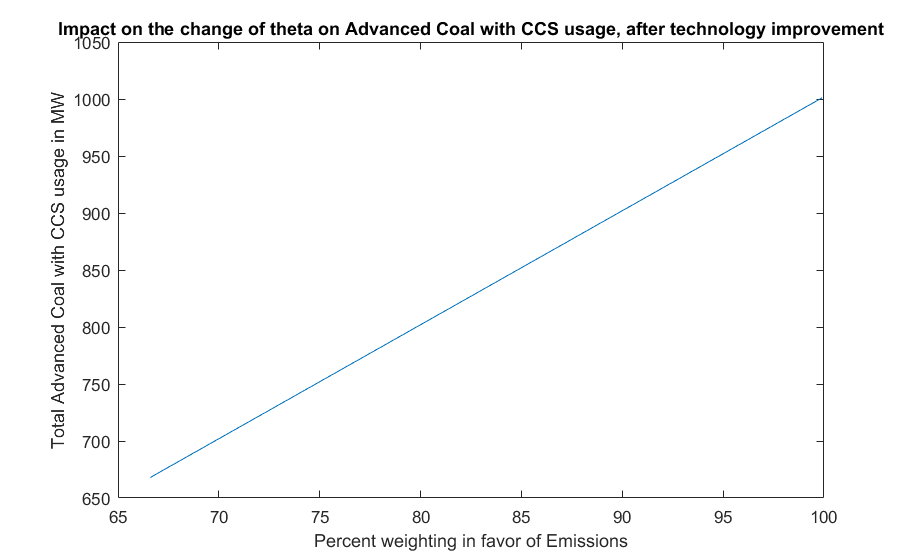
\includegraphics[width=\textwidth]{438_17_CCSvsTheta}
			\caption{Advanced Coal with Carbon Capture Storage Technology Advancement Analysis}
	\end{figure} 

	ACCCS was not used nor installed in the optimization of the total cost (Part 4.28). Although the capital cost of ACCCS is highly diminished by the technology break through, it is still almost three times higher than that of advanced CC natural gas, which is used to minimize cost as a peaker plant. The overarching conclusion is that the development on carbon storage has a significantly higher importance if emissions are a priority to the stakeholders, otherwise it is still an irrelevant option as it is not competitive financially.
	
	

%%%%%%%%%%%%%%%%%%%%%%%%%%%%%%%%%%%%
\paragraph{References}
[1] Ballotpedia. (2016). ``Washington Carbon Emission Tax and Sales Tax Reduction, Initiative 732 (2016).'' \textit{Ballotpedia}. \url{https://ballotpedia.org/Washington_Carbon_Emission_Tax_and_Sales_Tax_Reduction,_Initiative_732_(2016)} (Dec. 10, 2016).

[2] Porter, E. (2016). ``Does a Carbon Tax Work? Ask British Columbia.'' \textit{The New York Times}. \url{http://www.nytimes.com/2016/03/02/business/does-a-carbon-tax-work-ask-british-columbia.html?_r=0} (Dec. 10, 2016).

[3] Carbon Tax Center. (n.d.). ``British Columbia / Canada.'' \textit{Carbon Tax Center}. \url{https://www.carbontax.org/where-carbon-is-taxed/british-columbia/} (Dec. 10, 2016).

[4] Carbon Tax Center. (n.d.). ``Where Carbon Is Taxed'.'' \textit{Carbon Tax Center}. \url{https://www.carbontax.org/where-carbon-is-taxed/} (Dec. 10, 2016).

[5] U.S. Energy Information Administration. (2016). ``Electric Power Monthly, November 2016.'' \url{https://www.eia.gov/electricity/monthly/epm_table_grapher.cfm?t=epmt_5_6_a} (Dec. 11, 2016).

[6] Wood, L., Hemphill, R., Howat, J., Cavanagh, R., Borenstein, S. (2016). Recovery of Utility Fixed Costs: Utility, Consumer, Environmental and Economist Perspectives. Lawrence Berkeley Laboratory. \url{https://emp.lbl.gov/sites/all/files/lbnl-1005742_1.pdf}.


\end{document}